% !TeX root = main.tex

\section{État de l'art}
\label{sec:etat_art}

Ce chapitre passe en revue les technologies disponibles pour l'analyse automatique de documents. Pour chaque méthode, le fonctionnement, les résultats et les limites sont analysés afin de justifier les choix retenus pour la chaîne de traitement.

\subsection{La lecture de texte imprimé (OCR)}
\label{subsec:ocr}

La reconnaissance optique de caractères (OCR - \textit{Optical Character Recognition}) a été conçue pour automatiser la lecture de documents imprimés ou dactylographiés. L'objectif est de transformer une image de texte en caractères numériques exploitables par un ordinateur.

Le fonctionnement classique repose sur le découpage successif des éléments du document. L'image est d'abord binarisée pour séparer l'encre du papier. Le moteur repère ensuite les lignes de texte, puis découpe chaque ligne en mots et chaque mot en caractères isolés. Enfin, chaque caractère découpé est comparé à des modèles connus pour être identifié. Le moteur Tesseract illustre bien ce principe : pour repérer la ligne de base du texte même si la page est penchée ou courbée (comme près de la reliure d'un livre numérisé), il trace une ligne courbe mathématique (une spline quadratique) qui épouse l'ondulation des mots. Cela lui permet de lire le texte sans devoir redresser ou déformer l'image au préalable \citep{smith_tesseract_2007}.

Avec l'arrivée du deep learning, l'OCR n'a plus besoin de découper chaque caractère un par un. Les modèles modernes lisent la ligne entière d'un seul coup \citep{shi_crnn_2015}. \cite{baek_stract_2019} décomposent ce fonctionnement en quatre étapes principales, illustrées par la Figure~\ref{fig:ocr_pipeline} :

\begin{itemize}
  \item \textbf{La transformation géométrique (Trans.)} : normaliser la forme de la ligne de texte pour corriger les angles ou les déformations.
  \item \textbf{L'extraction de caractéristiques (Feat.)} : analyser les formes visuelles de l'image à l'aide d'un réseau de convolution (CNN).
  \item \textbf{La modélisation de séquence (Seq.)} : prendre en compte le contexte entre les lettres grâce à un réseau récurrent (BiLSTM).
  \item \textbf{La prédiction (Pred.)} : convertir la séquence visuelle en texte final grâce à une fonction d'alignement (CTC) ou d'attention.
\end{itemize}

\begin{figure}[H]
    \centering
    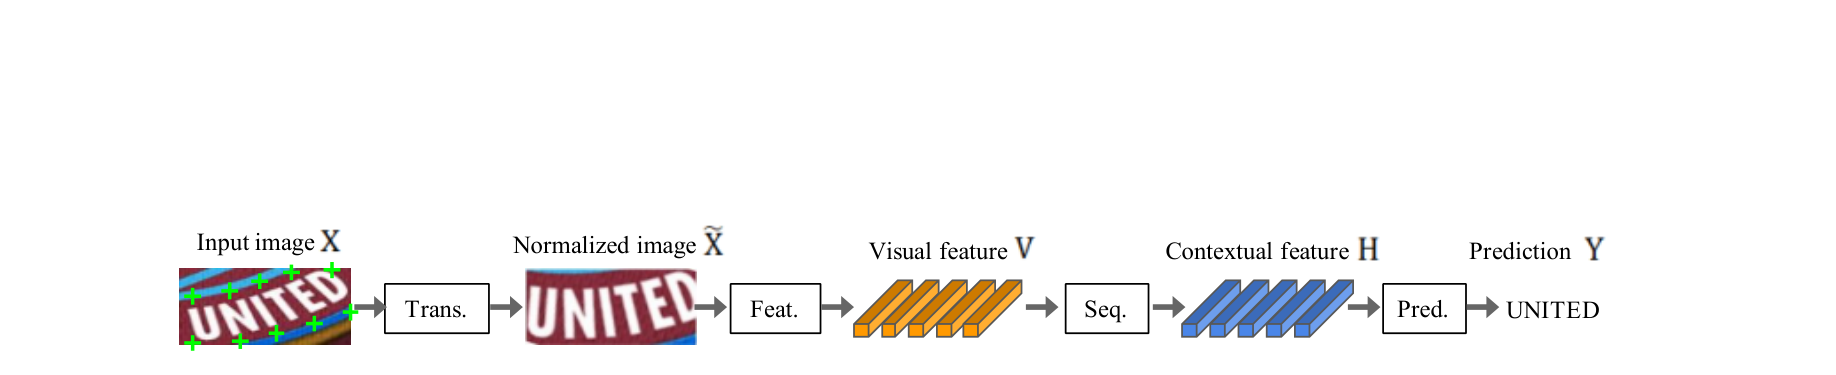
\includegraphics[width=\textwidth]{img/baek_ocr_pipeline_crop.png}
    \caption{Chaîne de reconnaissance de texte imprimé en quatre étapes : transformation géométrique (Trans.), extraction de caractéristiques visuelles (Feat.), modélisation de séquence (Seq.) et prédiction du texte (Pred.). Extrait de \cite{baek_stract_2019}.}
    \label{fig:ocr_pipeline}
\end{figure}

Cette méthode est fiable sur du texte imprimé ou dactylographié. En revanche, elle trouve sa limite sur l'écriture manuscrite, car le chevauchement des lettres empêche le modèle de distinguer les caractères correctement, et donc de trouver une correspondance avec son entraînement.

Pour surmonter les dégradations physiques des papiers anciens, les moteurs de numérisation s'appuient souvent sur des filtres de binarisation adaptative. La méthode d'Otsu cherche un seuil global optimal en minimisant la variance intra-classe des intensités de gris, ce qui fonctionne bien sur un fond homogène. Néanmoins, lorsque le document présente des taches d'humidité ou un jaunissement inégal, la binarisation de Sauvola calcule un seuil local pour chaque pixel en fonction de la moyenne et de l'écart-type de son voisinage. Ce traitement local préserve les traits fins des caractères imprimés sans amplifier les ombres de fond ou le bruit du papier.



\subsection{La reconnaissance de l'écriture manuscrite (HTR)}
\label{subsec:htr}

La reconnaissance de texte manuscrit (HTR - \textit{Handwritten Text Recognition}) a été conçue pour lire l'écriture à la main, sur laquelle l'OCR échoue. En écriture manuscrite, les lettres sont attachées, déformées et de tailles variables. Tenter de séparer chaque caractère individuellement provoque des erreurs systématiques. Pour résoudre ce problème, les systèmes HTR ne découpent pas les lettres : ils analysent la ligne entière comme un signal visuel continu.

La Figure~\ref{fig:rem_workflow} détaille le fonctionnement général de cette approche en trois étapes \citep{chague_htr-united_nodate} :

\begin{itemize}
  \item \textbf{La segmentation en lignes} : le système repère l'emplacement exact de chaque ligne de texte dans la page. Il trace une ligne de base (\textit{baseline}) sous l'écriture et extrait le masque d'image correspondant à la ligne.
  \item \textbf{L'analyse de la mise en page} : le modèle détermine l'ordre logique de lecture des différents blocs ou segments extraits de la page.
  \item \textbf{La transcription} : chaque portion d'image de ligne est convertie directement en une chaîne de caractères.
\end{itemize}

\begin{figure}[H]
    \centering
    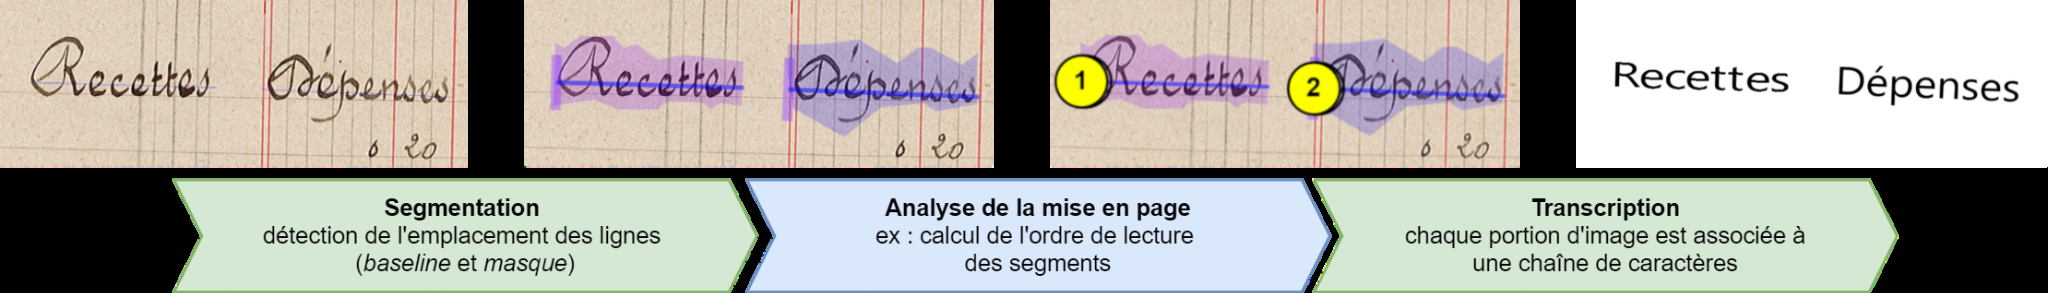
\includegraphics[width=\textwidth]{img/chague_fig1.png}
    \caption{Étapes de traitement d'un système HTR : segmentation de la page en lignes, analyse de la mise en page, puis transcription de chaque portion d'image en texte. Extrait de \cite{chague_htr-united_nodate}.}
    \label{fig:rem_workflow}
\end{figure}

Pour réaliser la phase de transcription, la littérature scientifique privilégie deux grandes architectures de réseaux de neurones.

La première repose sur l'alliance de réseaux de convolution et d'un alignement temporel (CNN + CTC), comme par exemple le modèle PyLaia \citep{tarride_improving_2024}. Des couches de convolution extraient d'abord la représentation visuelle de la ligne. Un réseau bidirectionnel (BLSTM) parcourt ensuite ces caractéristiques pour capter le contexte des mots. Enfin, la fonction de perte CTC (\textit{Connectionist Temporal Classification}) calcule la séquence de texte la plus probable sans imposer d'annoter la position exacte de chaque lettre dans l'image. Cette méthode présente l'avantage d'être légère en calcul et de bien s'entraîner sur des volumes restreints de données.

La seconde approche s'appuie sur l'architecture des Transformers, utilisée par le modèle TrOCR \citep{alkendi_advancements_2024}. L'image de la ligne est découpée en petits carrés visuels, appelés patchs. Un encodeur visuel (ViT) transforme ces patchs en vecteurs, qu'un décodeur de langage utilise pour générer le texte mot après mot. Le modèle calcule un poids visuel pour chaque région de l'image grâce au mécanisme d'attention issu de \cite{vaswani_attention_2017} et repris par \cite{alkendi_advancements_2024} :

\begin{equation}
  \text{Attention}(Q, K, V) = \text{softmax}\!\left(\frac{Q K^T}{\sqrt{d_k}}\right) V
\end{equation}

Dans cette formule, $Q$, $K$ et $V$ représentent les projections des patchs d'image sous forme de requêtes, de clés et de valeurs, et $d_k$ désigne la dimension des clés. Concrètement, le produit $Q K^T$ évalue la similitude entre le caractère recherché et chaque zone de l'image. La fonction \text{softmax} convertit ces scores en poids d'attention compris entre 0 et 1 : plus la correspondance entre la requête $Q$ et la clé $K$ est forte, plus le poids attribué à la valeur visuelle $V$ augmente. À chaque caractère généré, le réseau focalise ainsi son attention directement sur le tracé de la lettre correspondante. 
Sur des documents d'archives en français, ces modèles atteignent des taux d'erreur sur les caractères très faibles, inférieurs à 5~\% \citep{alkendi_advancements_2024, beatrice_challenges_2023}.

La principale contrainte du HTR est sa dépendance à la qualité du découpage des lignes. Si un tampon, une tache ou un élément de tableau vient couper le tracé d'une ligne, la phase de transcription perd en précision et génère des erreurs de lecture.

Pour bien comprendre la différence entre l'OCR et le HTR, présenté dans le chapitre précédent, elle repose sur le type de texte à lire et sur la façon dont le moteur l'analyse :

\begin{itemize}
  \item \textbf{L'OCR} s'applique au texte imprimé (\textit{Printed Text}). Comme les lettres sont régulières et séparées, le système cherche à isoler chaque caractère ou petit bloc avant de l'identifier.
  \item \textbf{Le HTR} s'applique à l'écriture manuscrite (\textit{Handwritten Text}). Comme les lettres sont attachées et varient selon les personnes, le système ne cherche pas à découper les caractères : il lit la ligne entière comme un tracé continu.
\end{itemize}

La Figure~\ref{fig:text_recognition_taxonomy} illustre cette séparation entre les technologies de reconnaissance de texte.

\begin{figure}[H]
    \centering
    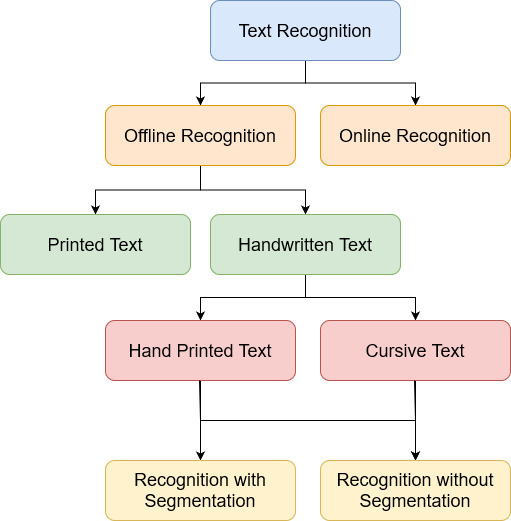
\includegraphics[width=0.55\textwidth]{img/fig_alkendi_p3_1.jpeg}
    \caption{Classification des systèmes de reconnaissance de texte : distinction entre le texte imprimé (\textit{Printed Text} / OCR) et le texte manuscrit (\textit{Handwritten Text} / HTR). Extrait de \cite{alkendi_advancements_2024}.}
    \label{fig:text_recognition_taxonomy}
\end{figure}

Cette arborescence résume la classification des systèmes de reconnaissance de texte. Elle sépare le traitement en deux branches : le traitement hors ligne sur des images scannées et le traitement en ligne en temps réel. Pour les images d'archives, la classification distingue le texte imprimé (OCR) et le texte manuscrit (HTR), qui nécessite une lecture globale sans découpage préalable des caractères.

Comme nous le verrons lors de la présentation de l'architecture (chapitre~\ref{sec:architecture}), le choix s'est porté sur une utilisation conjointe d'EasyOCR pour les parties imprimées et du modèle HTR PyLaia pour l'écriture manuscrite des anciens registres. PyLaia permet d'obtenir un compromis efficace entre rapidité d'exécution et autonomie locale, évitant ainsi d'alourdir les calculs sur les serveurs du cabinet.


Lorsque des documents associent texte imprimé et écriture manuscrite, des approches hybrides peuvent être envisagées.


\subsection{Les approches hybrides : OCR et HTR combinés}
\label{subsec:hybrid_ocr_htr}

En réalité, beaucoup de documents mélangent du texte imprimé et des ajouts écrits à la main, comme un formulaire pré-rempli. Un modèle OCR classique échoue sur les écritures manuscrites, tandis qu'un modèle HTR peut faire des erreurs sur du texte imprimé.

Pour résoudre ce problème, des approches hybrides ont été développées afin de traiter conjointement les deux types d'écriture. 

D'après la littérature scientifique, deux méthodes principales existent :

\begin{itemize}
  \item L'entraînement sur des exemples variés : le modèle TrOCR \citep{li_trocr_2021} s'appuie sur une architecture Transformer entraînée à la fois sur du texte imprimé et du texte écrit à la main. La Figure~\ref{fig:trocr_arch} montre ce principe : l'image de la ligne est découpée en petits carrés visuels (\textit{Image Patches}), convertis en vecteurs avec leur position, puis transmis à un encodeur visuel. Le décodeur produit ensuite le texte mot à mot. Comme le modèle a appris sur les deux formes d'écriture, il s'adapte tout seul sans étape de tri.
  \item La combinaison de deux outils successifs : des systèmes comme PaddleOCR \citep{du_ppocr_2020} ou EasyOCR utilisent un premier modèle pour repérer l'emplacement des lignes sur la page (comme DBNet \citep{liao_dbnet_2020}), puis un second modèle chargé uniquement de lire le texte présent dans ces zones.

\end{itemize}

\begin{figure}[H]
    \centering
    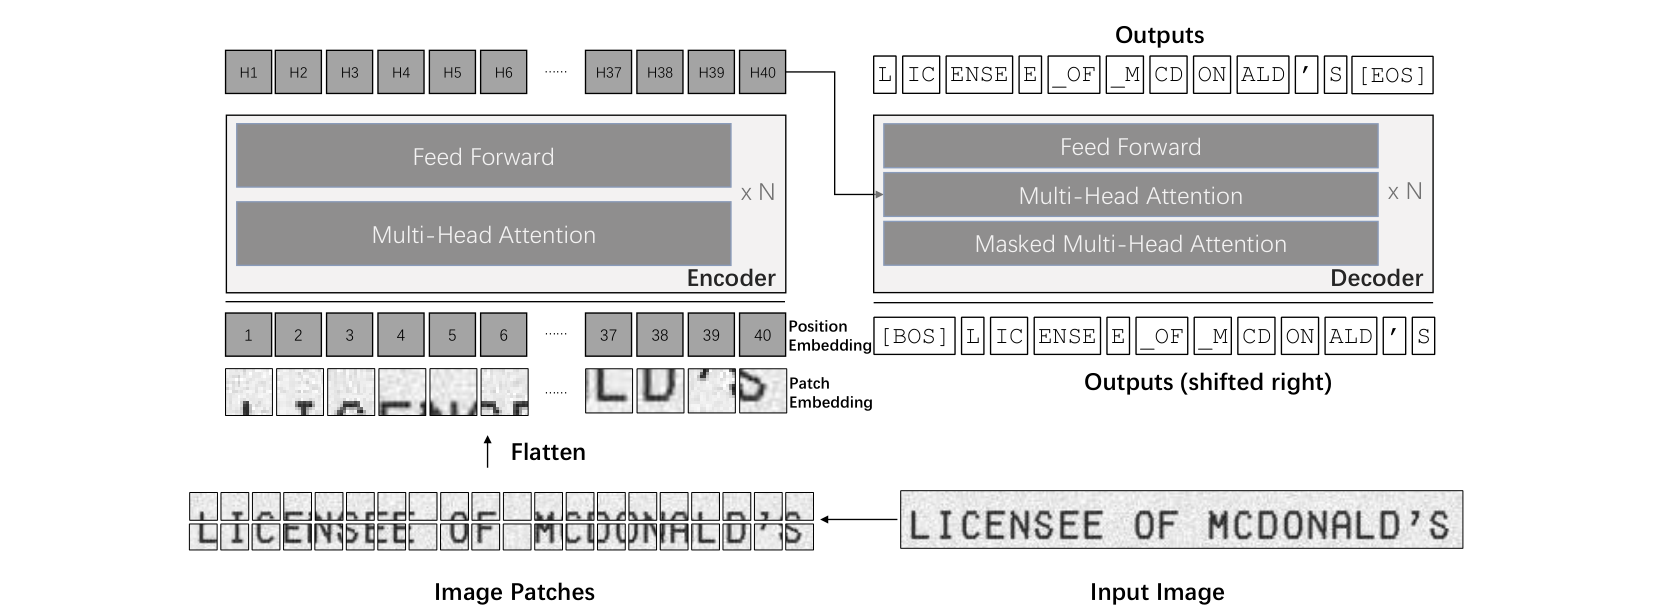
\includegraphics[width=\textwidth]{img/trocr_architecture_crop.png}
    \caption{Architecture hybride de TrOCR : l'image de la ligne (imprimée ou manuscrite) est découpée en patchs visuels traités par un encodeur Transformer, puis transcrite par un décodeur de texte. Extrait de \cite{li_trocr_2021}.}
    \label{fig:trocr_arch}
\end{figure}

Le principal avantage de ces approches hybrides est leur polyvalence. Un seul modèle traite l'ensemble des contenus de la page sans tri par un opérateur. En contrepartie, ces réseaux sont plus lourds car ils comptent plusieurs centaines de millions de paramètres \citep{li_trocr_2021}. Leur exécution nécessite donc une carte graphique (GPU) pour conserver une vitesse de lecture rapide.

Quelle que soit l'approche retenue (OCR, HTR ou hybride), envoyer une page entière au modèle de reconnaissance reste inefficace : la présence de tampons, de marges ou de cadres perturbe la lecture. Il est donc nécessaire de repérer d'abord les zones d'intérêt dans la page avant de lancer la transcription.




\subsection{La détection spatiale et l'analyse de mise en page par YOLO}

Envoyer directement la photo complète d'un document à un moteur de lecture pose un problème : la page contient des marges blanches, des tampons, des lignes de cadres et des annotations. Si le moteur essaie de tout lire sans tri, ce dernier perd du temps et produit du texte parasite. Il est donc important d'isoler d'abord les zones d'intérêt dans la page avant d'extraire le texte.

Le modèle YOLO (\textit{You Only Look Once}) \citep{redmon_yolo_2016, jiang_review_2022} a été conçu pour détecter des objets et des zones visuelles en un seul passage rapide sur l'image.

\begin{figure}[H]
    \centering
    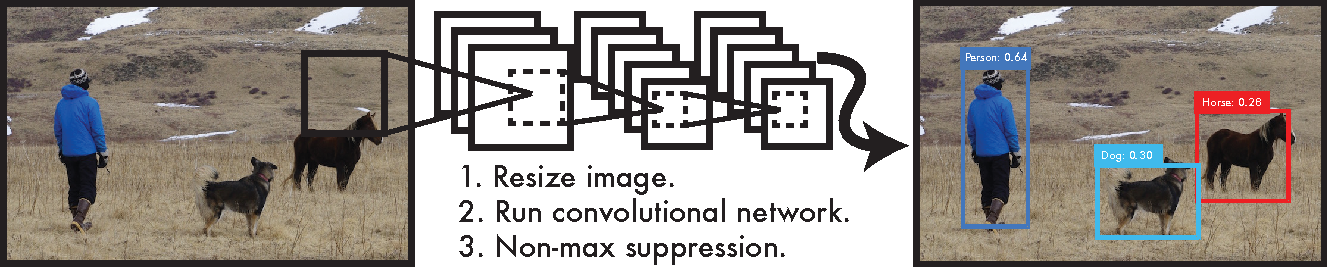
\includegraphics[width=0.8\textwidth]{img/yolo_system.pdf}
    \caption{Principe de détection de YOLO : traitement en un seul passage (\textit{Single-Shot}) sur une grille spatiale. Extrait de \cite{redmon_yolo_2016}.}
    \label{fig:yolo_architecture}
\end{figure}

La Figure~\ref{fig:yolo_architecture} illustre ce procédé. Dans un premier temps, l'image complète du document est redimensionnée pour être analysée d'un seul coup. Le réseau divise ensuite la page en une grille de cellules et calcule simultanément la position des boîtes englobantes et leur catégorie. Enfin, un filtre d'élimination des doublons (\textit{Non-Max Suppression}) ne conserve que le cadre le plus précis autour de chaque zone.

Pour garantir un bon cadrage cases et des tableaux, l'entraînement de YOLOv8 utilise la fonction de perte CIoU (\textit{Complete Intersection over Union}) \citep{zheng_ciou_2020} :

\begin{equation}
  \mathcal{L}_{CIoU} = 1 - IoU + \frac{\rho^2(\mathbf{b}, \mathbf{b}^{gt})}{c^2} + \alpha v
\end{equation}

Cette formule mesure la qualité du cadrage selon trois critères : le chevauchement ($IoU$) entre la boîte prédite et la vraie zone, l'écart de distance ($\rho^2 / c^2$) entre leurs centres respectifs, et la cohérence de la forme ($\alpha v$) pour préserver les proportions en hauteur et en largeur. Concrètement, l'entraînement cherche à réduire cette perte $\mathcal{L}_{CIoU}$ vers 0. Lorsque le chevauchement $IoU$ augmente, le terme $1 - IoU$ diminue. À l'inverse, si la distance $\rho$ entre les centres s'agrandit ou si les proportions se déforment (hausse de $v$), la perte augmente et pénalise le modèle, l'obligeant à recentrer le cadre et ajuster ses dimensions. Grâce à cette astuce, YOLOv8 ajuste le contour des zones, même lorsqu'il s'agit de lignes fines ou de petites cases.

Pour comprendre comment le réseau extrait ces caractéristiques visuelles étape par étape avant d'ajuster les cadrages, la Figure~\ref{fig:yolo_net} présente l’architecture du modèle.

\begin{figure}[H]
    \centering
    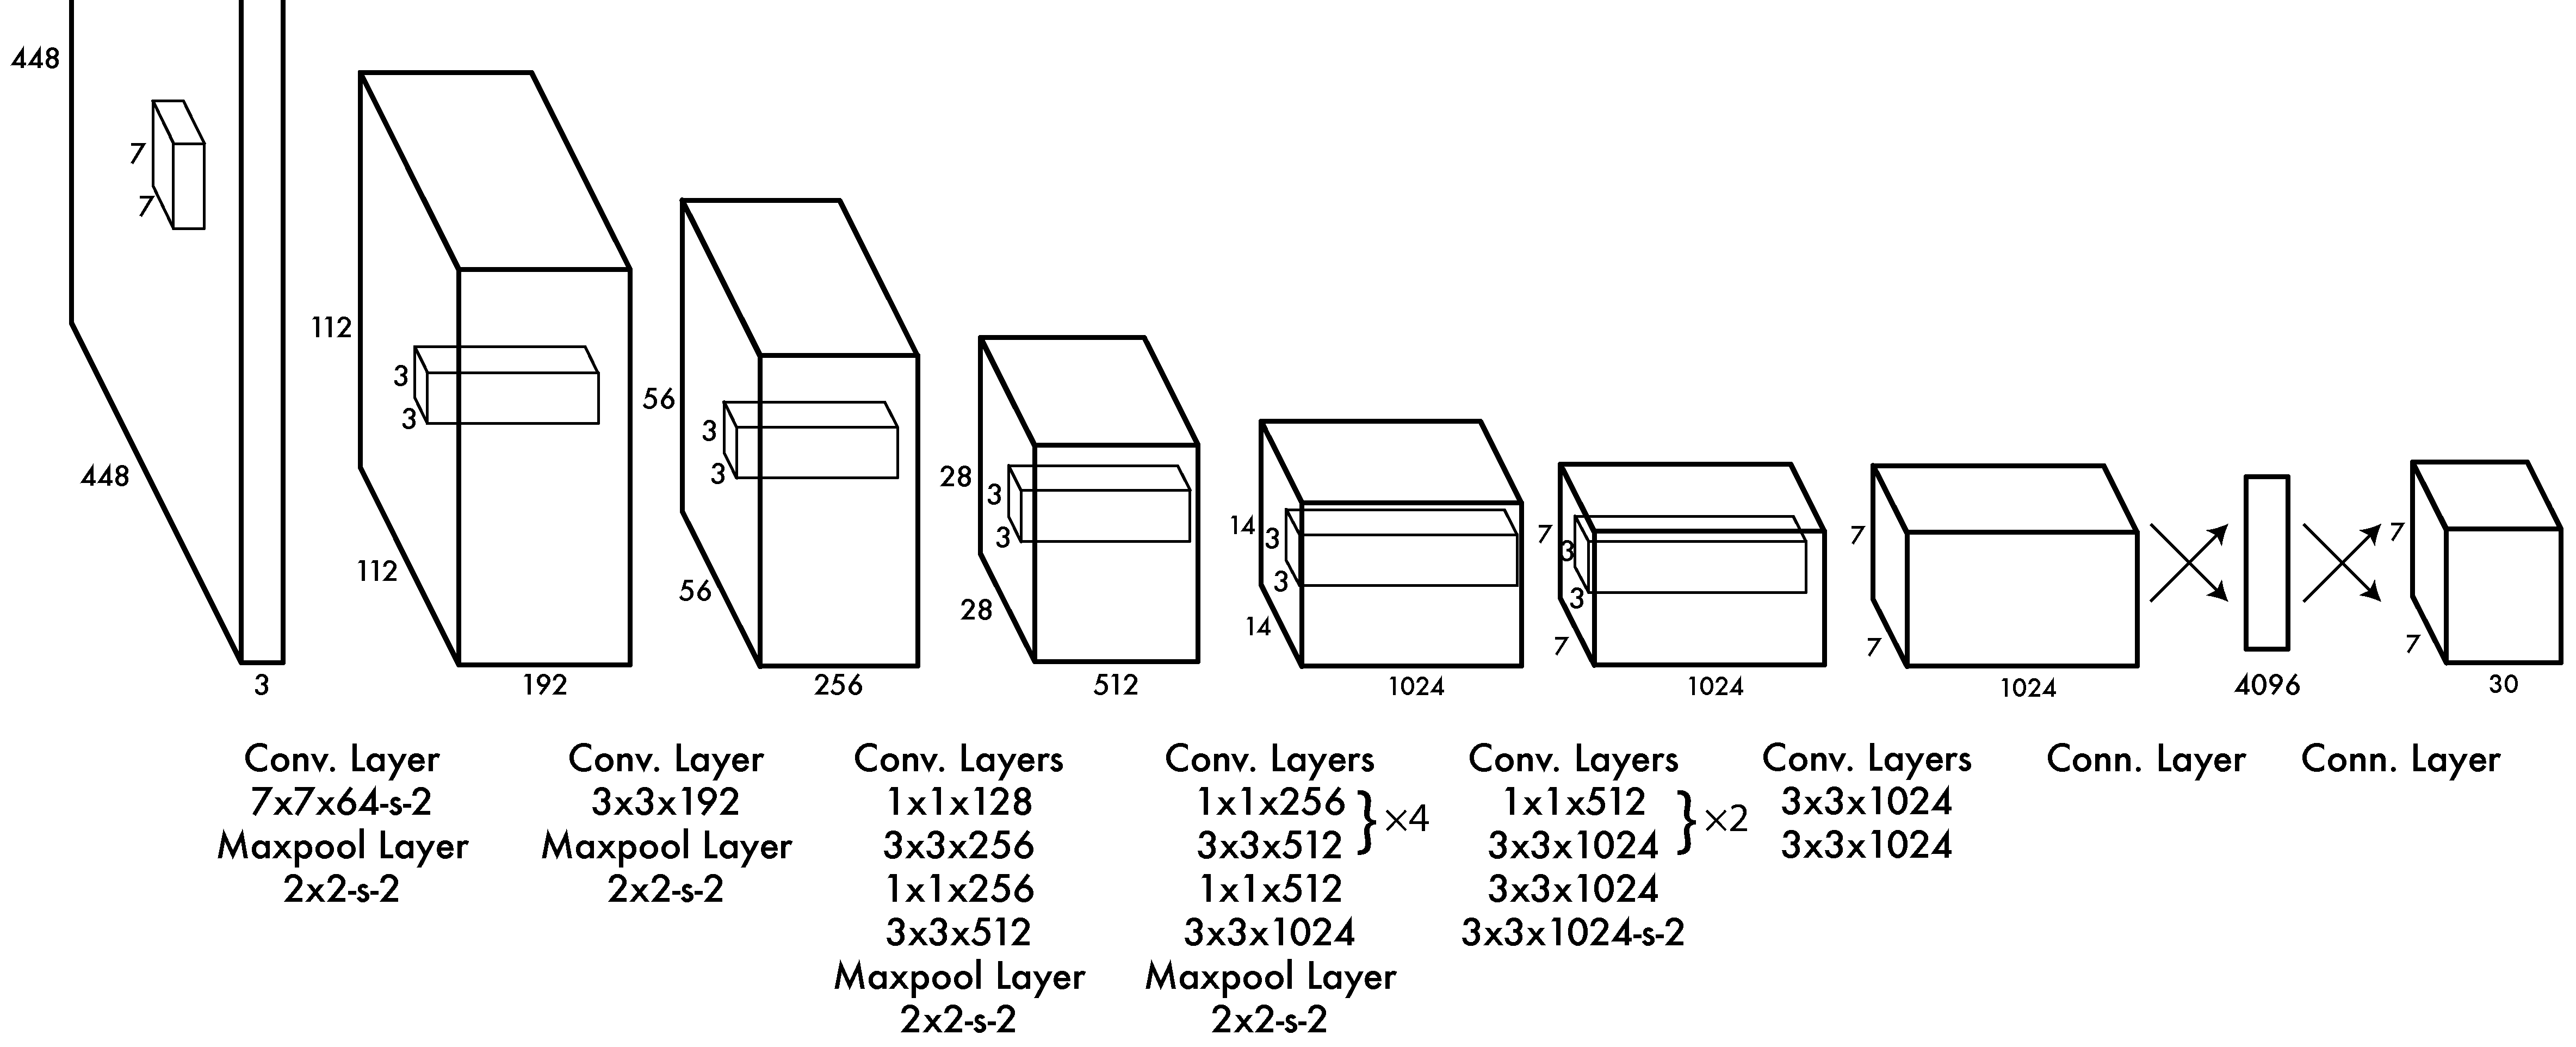
\includegraphics[width=\textwidth]{img/yolo_net.pdf}
    \caption{Architecture du réseau de convolution de YOLO. Extrait de \cite{redmon_yolo_2016}.}
    \label{fig:yolo_net}
\end{figure}

L'organisation du réseau de convolution responsable de la détection visuelle y est détaillée. L'image du document traverse d'abord une succession de couches de convolution qui repèrent les détails géométriques simples, pouvant être les lignes des tableaux, les angles ou encore les contours des cadres. Les couches suivantes combinent ces éléments pour reconnaître des blocs plus complexes, tels que des entêtes, des colonnes ou des cartouches. En parallèle, des opérations de sous-échantillonnage (\textit{max-pooling}) réduisent la taille spatiale pour préserver une vue globale sans alourdir les calculs. Enfin, les dernières couches du réseau convertissent ces caractéristiques visuelles en coordonnées spatiales(position, largeur et hauteur) et attribuent une catégorie à chaque zone identifiée.

Cette architecture permet à YOLO d'analyser rapidement la géométrie d'une page entière et d'isoler les zones d'intérêt.

Contrairement aux approches par modèles de détection classiques reposant sur des boîtes d'ancres pré-définies (*anchor-based*), la version v8 de YOLO utilise une architecture sans ancres (*anchor-free*). Ce choix simplifie l'apprentissage sur des documents administratifs aux formats non standard, car le réseau prédit directement les coordonnées du centre et les dimensions de chaque zone au lieu d'ajuster des cadres pré-formés. Sur des archives foncières où l'échelle des cartouches et l'emplacement des formulaires varient selon l'époque et l'imprimeur, cette flexibilité permet de détecter les zones utiles avec une meilleure précision qu'un simple découpage à coordonnées fixes.

Comme détaillé ultérieurement lors de l'explication de la chaîne de traitement (chapitre~\ref{sec:architecture}), cette étape de découpage spatial constitue le point d'entrée de toute l'analyse : elle préserve la mémoire de calcul en évitant de soumettre l'intégralité des images haute résolution aux modèles de lecture manuscrite.




Plutôt que de se reposer uniquement sur l'aspect visuel de la page comme YOLO, une autre approche consiste à utiliser des modèles multimodaux, capables de croiser le texte, la position des mots et l'image, comme par exemple LayoutLM \citep{xu_layoutlm_2020}.

\begin{figure}[H]
    \centering
    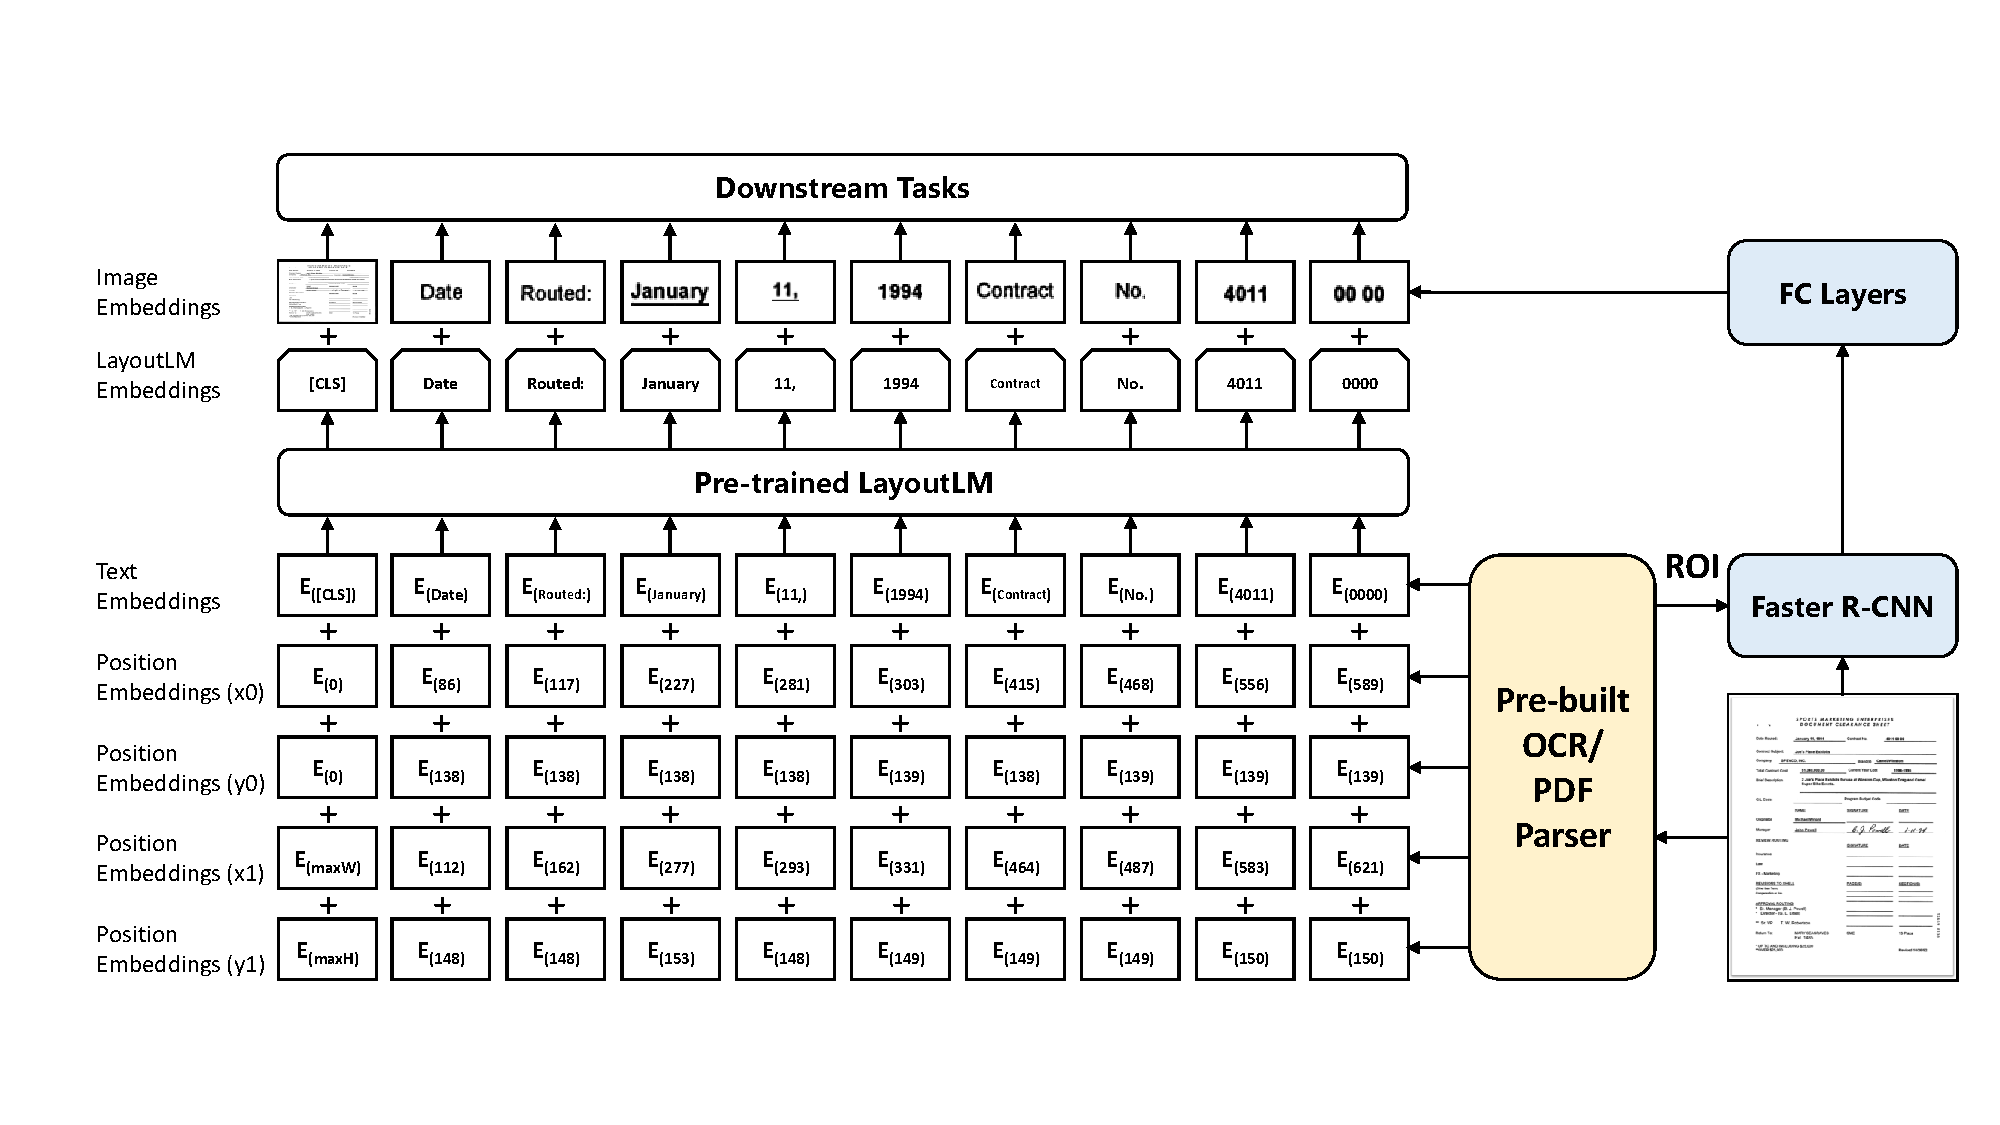
\includegraphics[width=\textwidth]{img/layoutlm_arch.pdf}
    \caption{Architecture de LayoutLM : combinaison du texte lu, de la position spatiale des mots sur la page et du signal visuel. Extrait de \cite{xu_layoutlm_2020}. Ce schéma est également disponible en grand format horizontal en \hyperref[ann:layoutlm]{Annexe B}.}
    \label{fig:layoutlm_architecture}
\end{figure}

Comme l'illustre le schéma de la Figure~\ref{fig:layoutlm_architecture}, ce modèle traite la page en faisant communiquer plusieurs canaux d'informations qui apparaissent à différents niveaux du diagramme.



En bas à droite du schéma, le document passe d'abord dans un moteur OCR préalable. Cet outil extrait les mots individuels (comme Date, January ou 1994) et calcule leurs coordonnées exactes sur la feuille, représentées par les quatre coins du cadre englobant $(x_0, y_0, x_1, y_1)$.

Au centre de l'architecture, chaque mot est transformé en un vecteur de texte (\textit{Text Embeddings}), auquel le modèle additionne directement quatre vecteurs de position (\textit{Position Embeddings}). Ces représentations spatiales indiquent où se situe le mot horizontalement et verticalement sur la page, ce qui permet au réseau Transformer (\textit{Pre-trained LayoutLM}) de comprendre la disposition en colonnes ou en tableaux.

En haut à droite du schéma, un réseau visuel (\textit{Faster R-CNN}) découpe l'image de chaque bloc pour extraire des caractéristiques visuelles (\textit{Image Embeddings}), comme la police d'écriture ou la présence de cadres. Ces informations visuelles sont ensuite ajoutées aux vecteurs de texte et de position pour produire la représentation finale du document.

Toutefois, cette architecture présente un point faible visible dès le début du schéma : la toute première brique repose entièrement sur le moteur OCR. Si cette lecture initiale échoue sur du texte manuscrit, des ratures ou une faible résolution, les mots transmis à la base de l'architecture sont erronés. Ces erreurs de texte se propagent ensuite dans tout le réseau Transformer et faussent la compréhension globale de la mise en page.

Pour mesurer l'impact de ces erreurs de texte sur les performances de LayoutLM, il est intéressant d'examiner la matrice de confusion mesurée par les auteurs du modèle (Figure~\ref{fig:layoutlm_confusion}).



\begin{figure}[H]
    \centering
    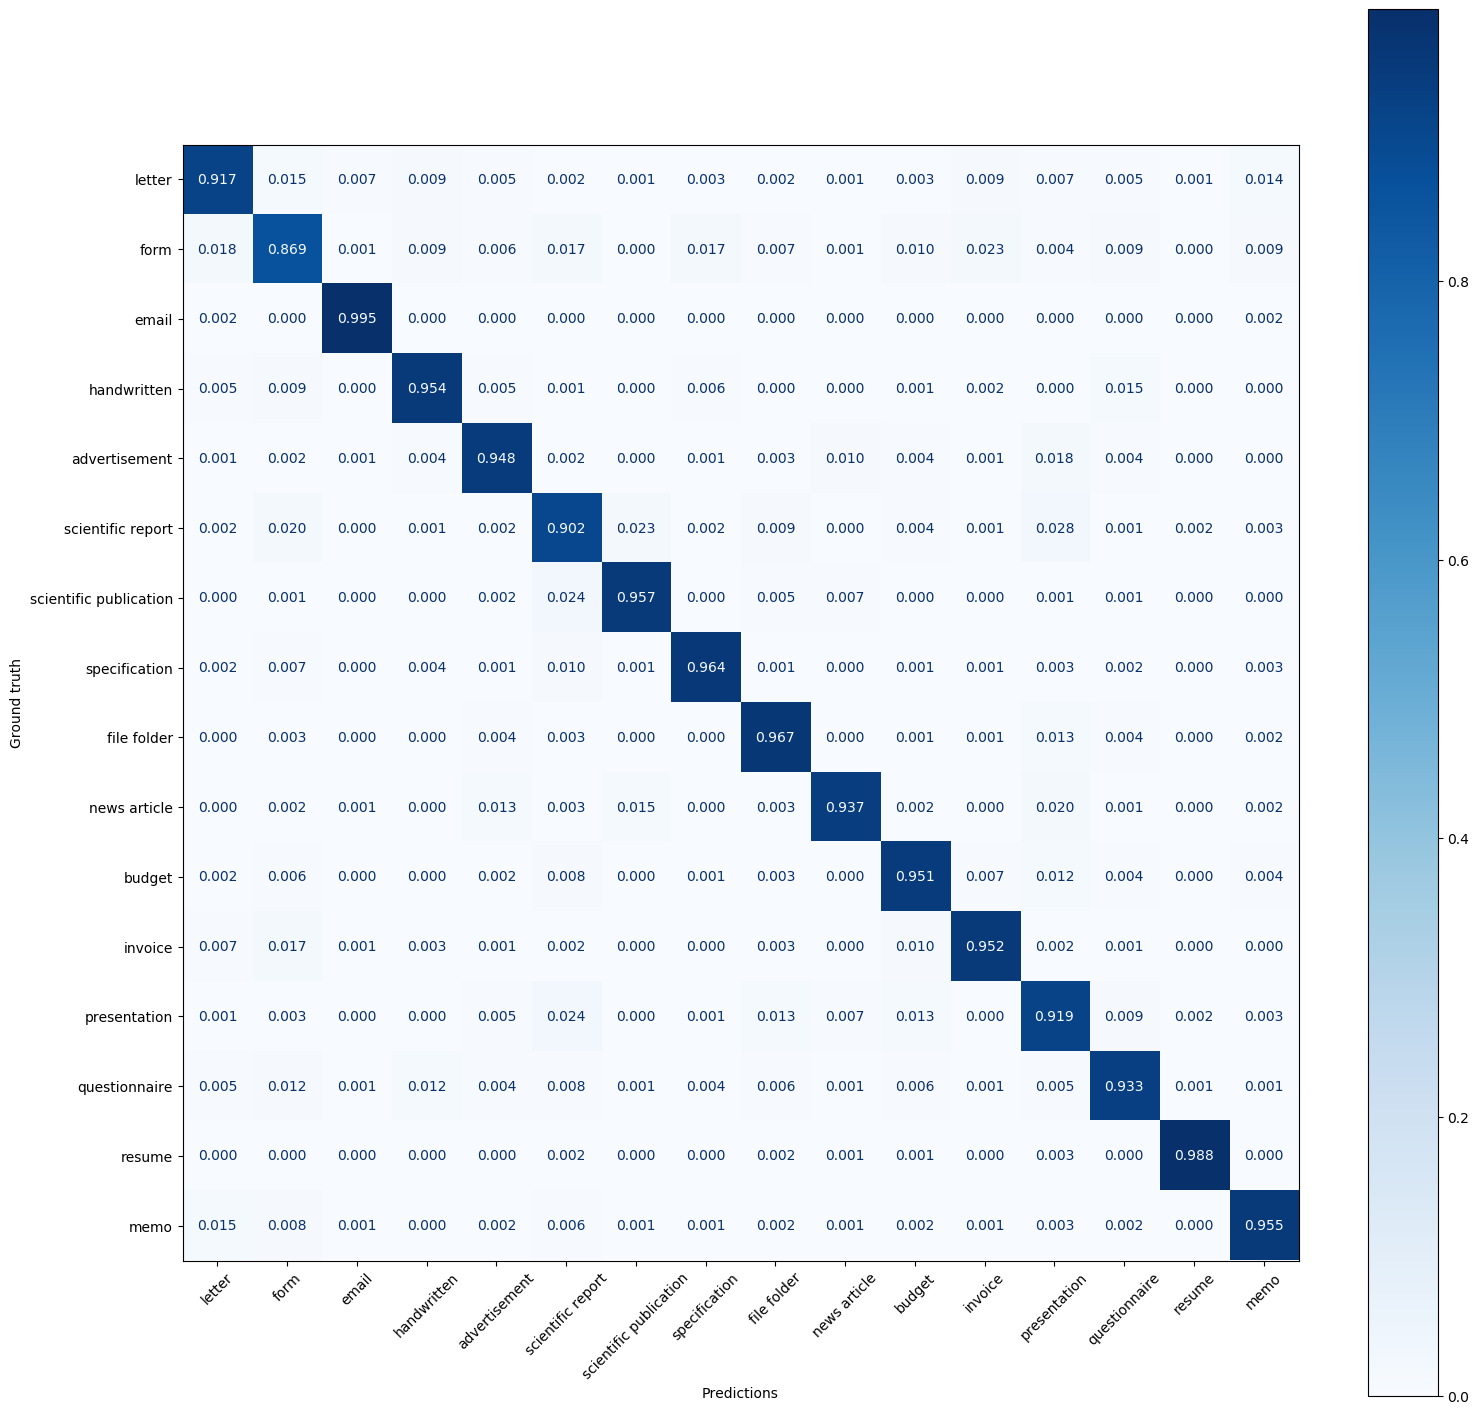
\includegraphics[width=0.65\textwidth]{img/layoutlm_confusion.png}
    \caption{Matrice de confusion de LayoutLM : la diagonale montre le taux de réussite pour chaque type de document, tandis que les cases hors diagonale révèlent les confusions causées par du texte mal reconnu. Extrait de \cite{xu_layoutlm_2020}. Cette matrice est également disponible en grand format horizontal en \hyperref[ann:layoutlm_confusion]{Annexe C}.}
    \label{fig:layoutlm_confusion}
\end{figure}


La Figure~\ref{fig:layoutlm_confusion} présente la matrice de confusion de LayoutLM. Ce tableau croisé permet d'analyser la précision du modèle en comparant la vraie catégorie de chaque document (affichée sur l'axe vertical) avec la catégorie prédite par le réseau (sur l'axe horizontal). Les cases situées sur la diagonale principale représentent les classements corrects, le bleu devenant plus foncé lorsque le score se rapproche de 1 (soit 100~\% de réussite).

L'observation de cette matrice met en évidence deux comportements très différents selon la nature des documents.

Dans les évolutions ultérieures comme LayoutLMv3, les auteurs ont simplifié cette architecture en supprimant la dépendance envers un moteur OCR externe pour l'étape d'analyse visuelle. LayoutLMv3 découpe directement la page scannée en petits patchs d'images (de taille 16 par 16 pixels) traités par un transformateur visuel (Vision Transformer), tout en alignant conjointement les jetons de texte et les positions spatiales. Cependant, cette avancée exige un volume d'entraînement considérable sur plusieurs millions de documents annotés. Pour des cabinets de géomètres disposant de fonds d'archives spécifiques et hétérogènes, le coût de réentraînement complet de telles architectures reste hors de portée par rapport à des approches plus modulaires.


D'une part, sur des documents imprimés comme les e-mails (99,5~\%), les CV (98,8~\%) ou les dossiers (96,7~\%), le modèle atteint d'excellents résultats. Dans ces cas, les mots reconnus par l'OCR (comme des entêtes d'e-mail ou des sections de CV) fournissent des repères fiables.

D'autre part, les performances diminuent sur des documents comme les formulaires (86,9~\%), les rapports scientifiques (90,2~\%) ou les courriers manuscrits (91,7~\%). Par exemple, la matrice indique que 2,3~\% des formulaires sont confondus avec des factures et 1,8~\% avec des courriers. Même si ces pourcentages d'erreur semblent faibles au premier abord, ils représentent rapidement une source d'erreur, ce qui peut nécessiter des corrections. 


Cette baisse de précision s'explique par la dépendance du modèle au texte. Lorsqu'un formulaire comporte des ajouts écris à la main, des cases cochées de manière irrégulière ou du texte dégradé, l'OCR préalable commet de nombreuses erreurs de lecture. En recevant ce texte bruité ou incomplet, le réseau de neurones de LayoutLM interprète mal la structure de la page et attribue le document à une mauvaise catégorie.

À l'inverse, un modèle de détection visuelle comme YOLO s'appuie uniquement sur la géométrie de la page (les lignes, les cadres et les colonnes) sans dépendre de la lecture du texte. Il n'est donc pas sensible à la présence d'écriture manuscrite ou de ratures pour repérer les blocs d'un document.








L'étape suivante consiste à passer du texte brut lu sur la page à une information structurée et exploitable.

\subsection{L'extraction d'entités et compréhension du texte}

Cette opération, appelée extraction d'entités nommées (NER pour \textit{Named Entity Recognition}), consiste à associer chaque mot ou groupe de mots à une catégorie précise.


Les outils de NER traditionnels (comme SpaCy ou CamemBERT) fonctionnent avec une liste fermée de catégories définies au moment de leur entraînement. Pour ajouter de nouvelles catégories spécifiques à un domaine, il faut annoter à la main des fichiers exemples puis réentraîner le modèle, ce qui demande du temps.

Pour contourner cette contrainte, le modèle GLiNER proposé par \citet{zaratiana_gliner_2024} introduit une approche capable de reconnaître de nouvelles catégories sur n'importe quel texte sans réentraînement préalable.

\begin{figure}[H]
    \centering
    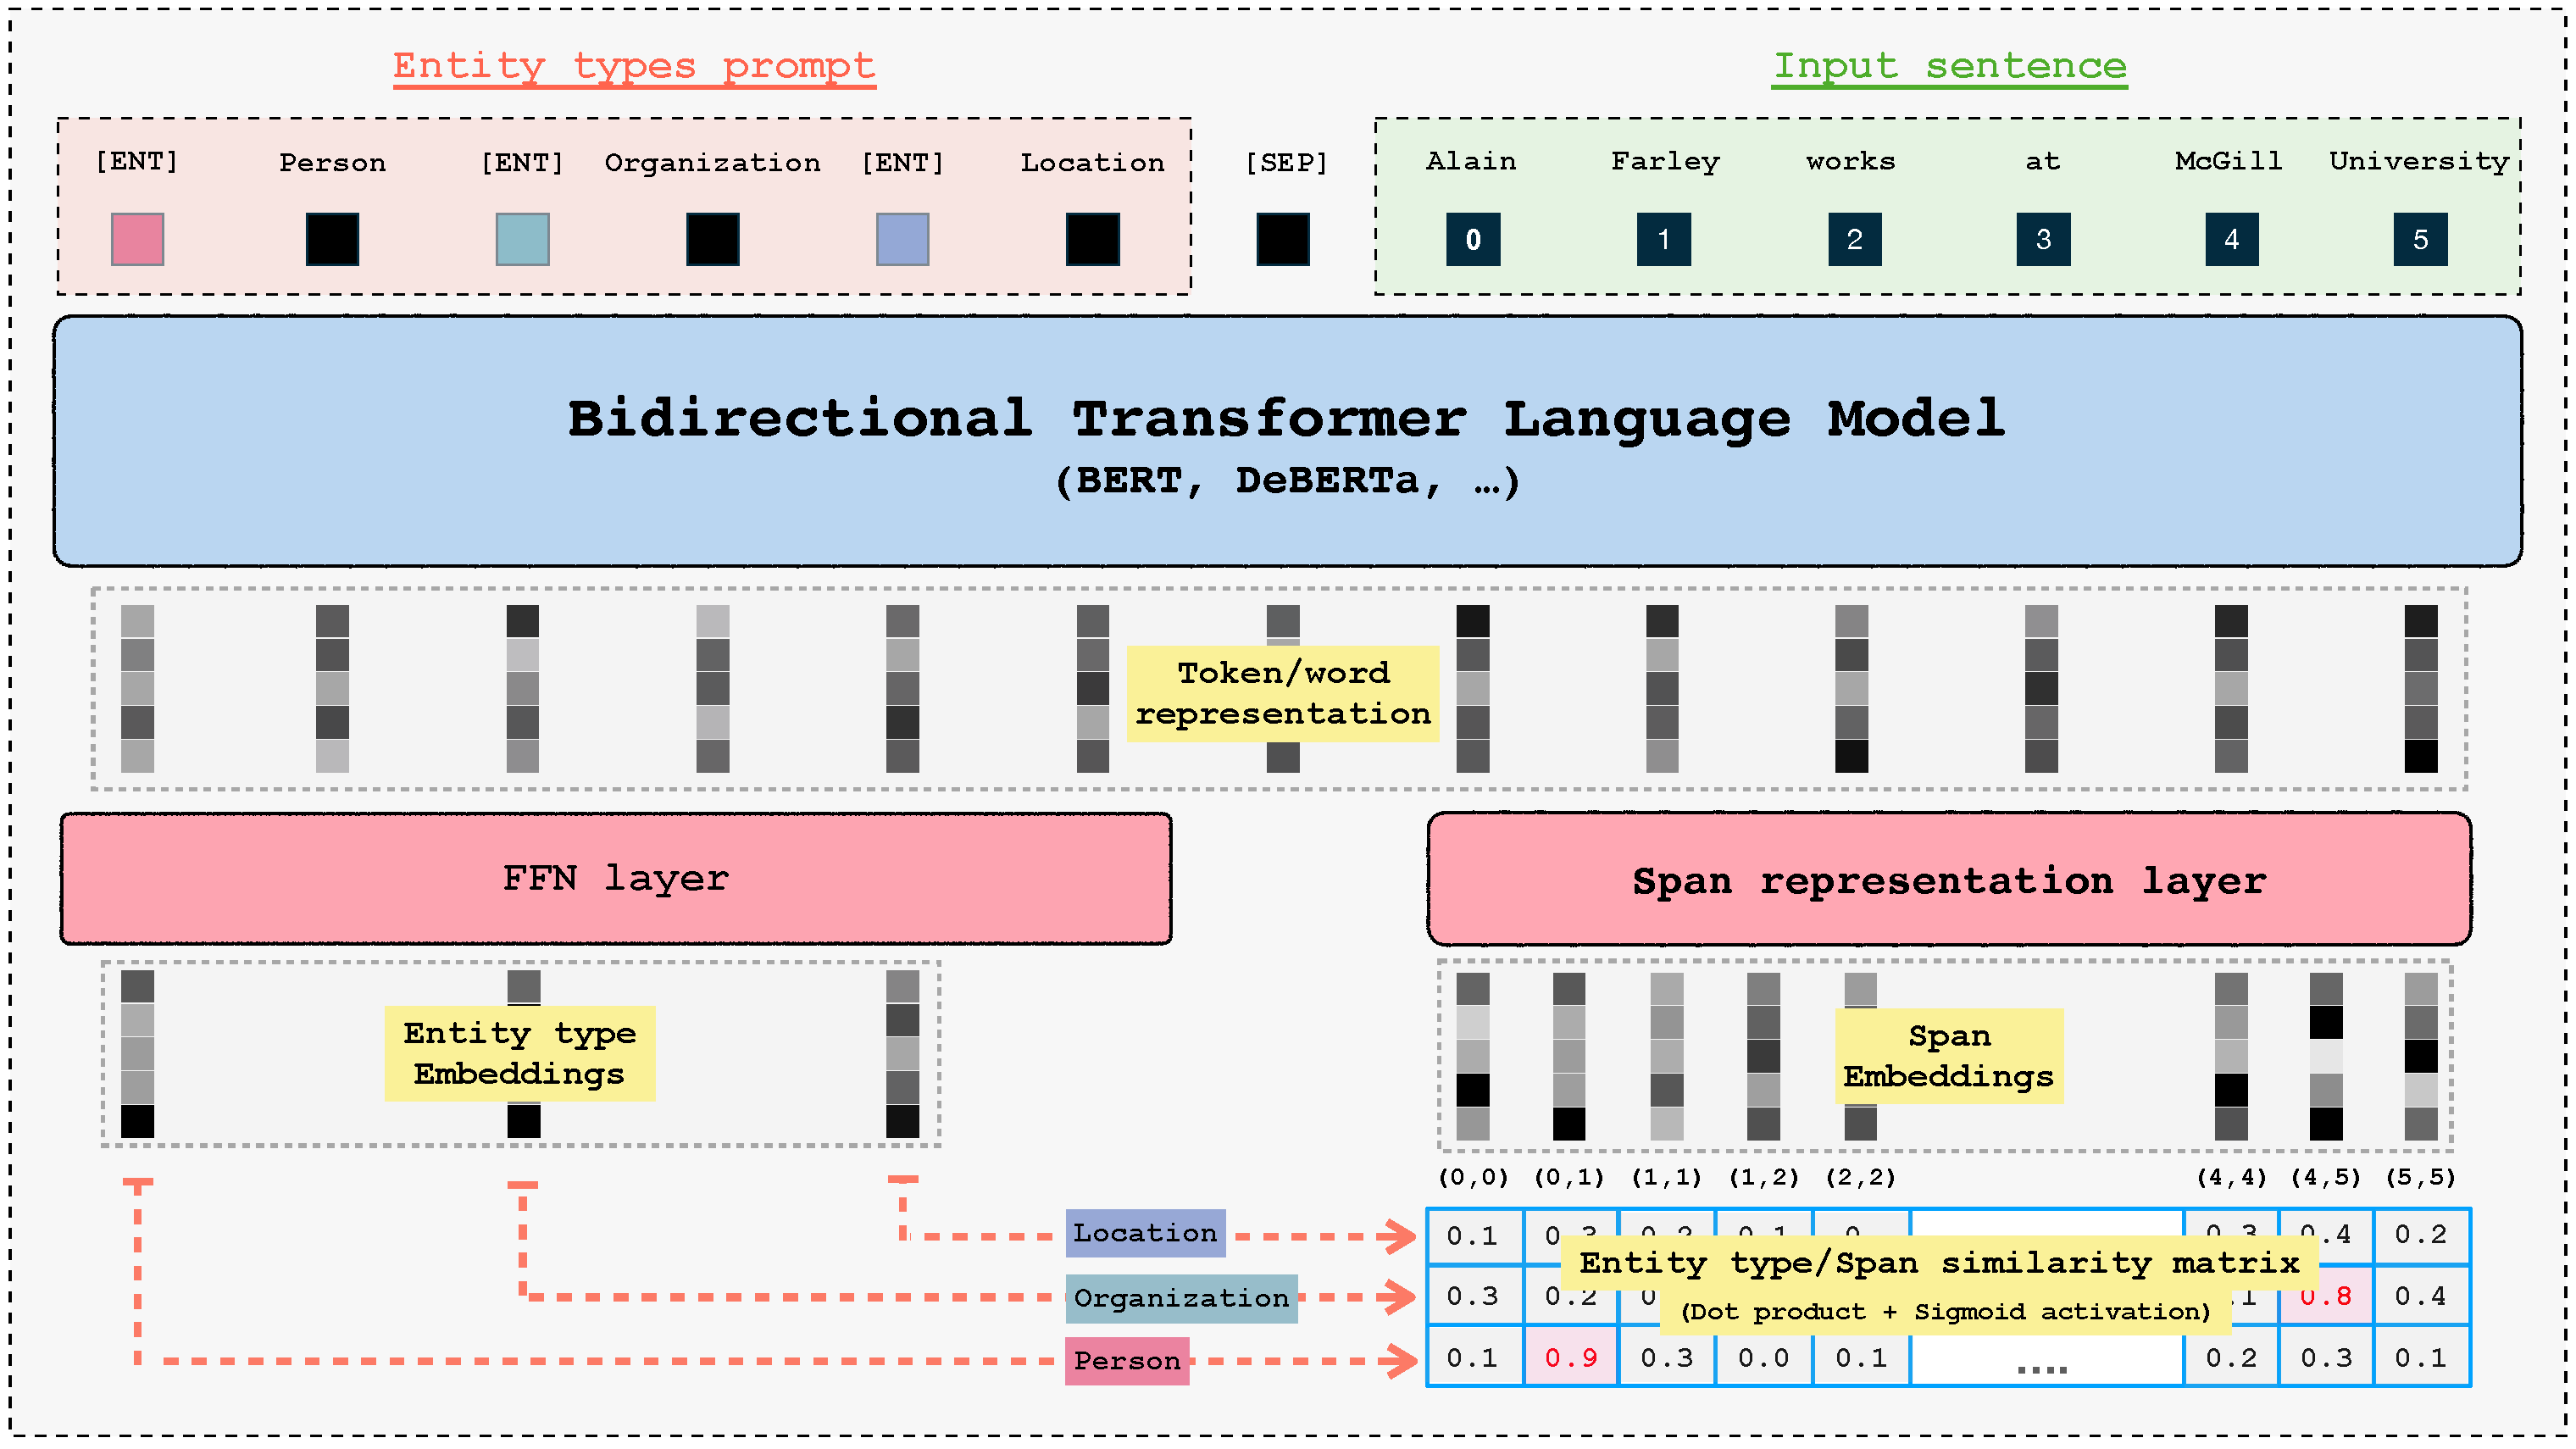
\includegraphics[width=0.9\textwidth]{img/gliner_gener.pdf}
    \caption{Architecture globale du modèle GLiNER : comparaison entre les morceaux de texte et les entités recherchées. Extrait de \cite{zaratiana_gliner_2024}. Ce schéma est également disponible en grand format horizontal en \hyperref[ann:gliner_architecture]{Annexe D}.}
    \label{fig:gliner_architecture}
\end{figure}

La Figure~\ref{fig:gliner_architecture} détaille l'organisation de ce réseau à travers plusieurs traitement.

En haut du schéma, le modèle reçoit deux entrées distinctes. À gauche, la consigne définit la liste des catégories recherchées (comme personne, organisation ou lieu), séparées par des balises. À droite, la phrase d'entrée contient le texte brut à analyser (par exemple \textit{Alain Farley works at McGill University}).

Au centre du schéma, l'ensemble traverse un modèle de langage bidirectionnel (comme DeBERTa). Ce réseau convertit simultanément la phrase et la liste des catégories en vecteurs numériques pour prendre en compte le contexte complet de chaque mot.

En bas du schéma, deux couches de projection calculent les caractéristiques finales. La branche de gauche produit la représentation numérique des catégories, tandis que la branche de droite regroupe les mots successifs en segments de texte, comme le nom complet \textit{Alain Farley}.

Enfin, le tableau bleu au bas de la figure présente la matrice de ressemblance. Le modèle calcule un produit scalaire entre chaque segment de texte et chaque catégorie recherchée. Dans l'exemple du schéma, le segment \textit{Alain Farley} s'associe à la catégorie des personnes avec un score élevé de 0,9, tandis que \textit{McGill University} correspond à la catégorie des organisations avec un score de 0,8.


Pour mettre en œuvre l'extraction d'entités avec GLiNER, deux facteurs doivent être pris en compte : la manière de formuler la consigne d'extraction et le choix du modèle de langage sous-jacent.

\begin{figure}[H]
    \centering
    \begin{minipage}{0.48\textwidth}
        \centering
        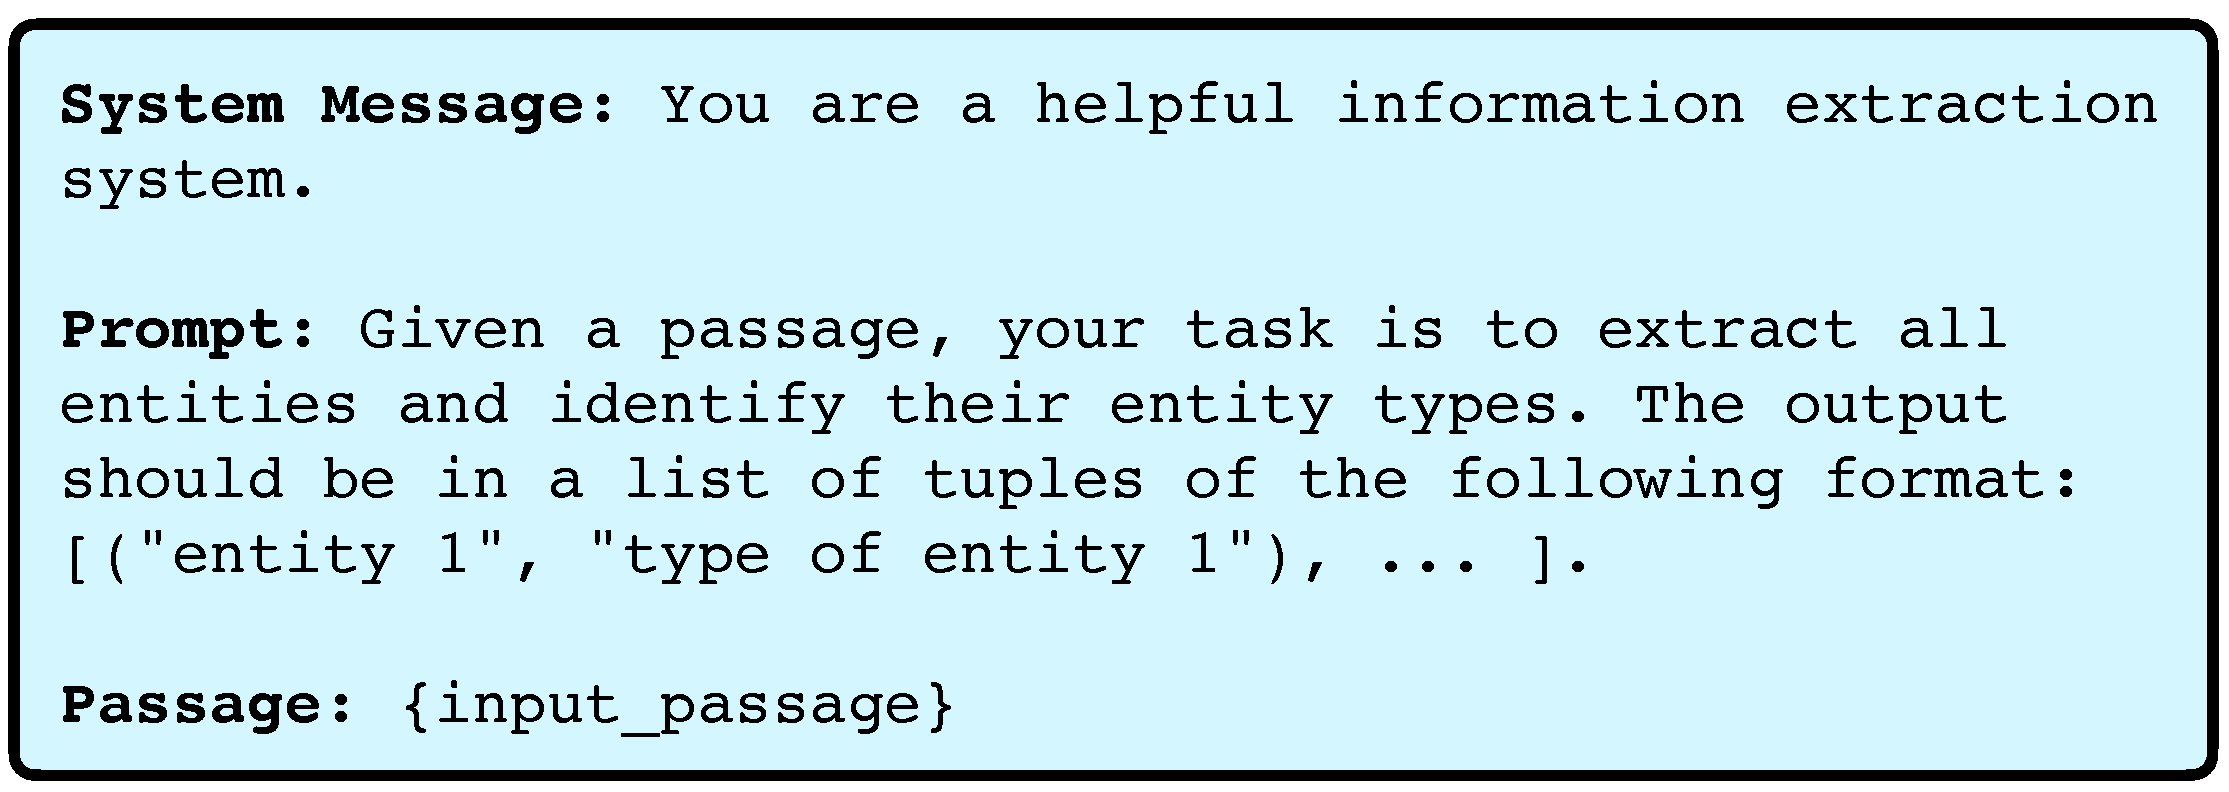
\includegraphics[width=\linewidth]{img/gliner_prompt.pdf}
        \caption{Format de la consigne transmise au modèle. Extrait de \cite{zaratiana_gliner_2024}.}
        \label{fig:gliner_prompt}
    \end{minipage}\hfill
    \begin{minipage}{0.48\textwidth}
        \centering
        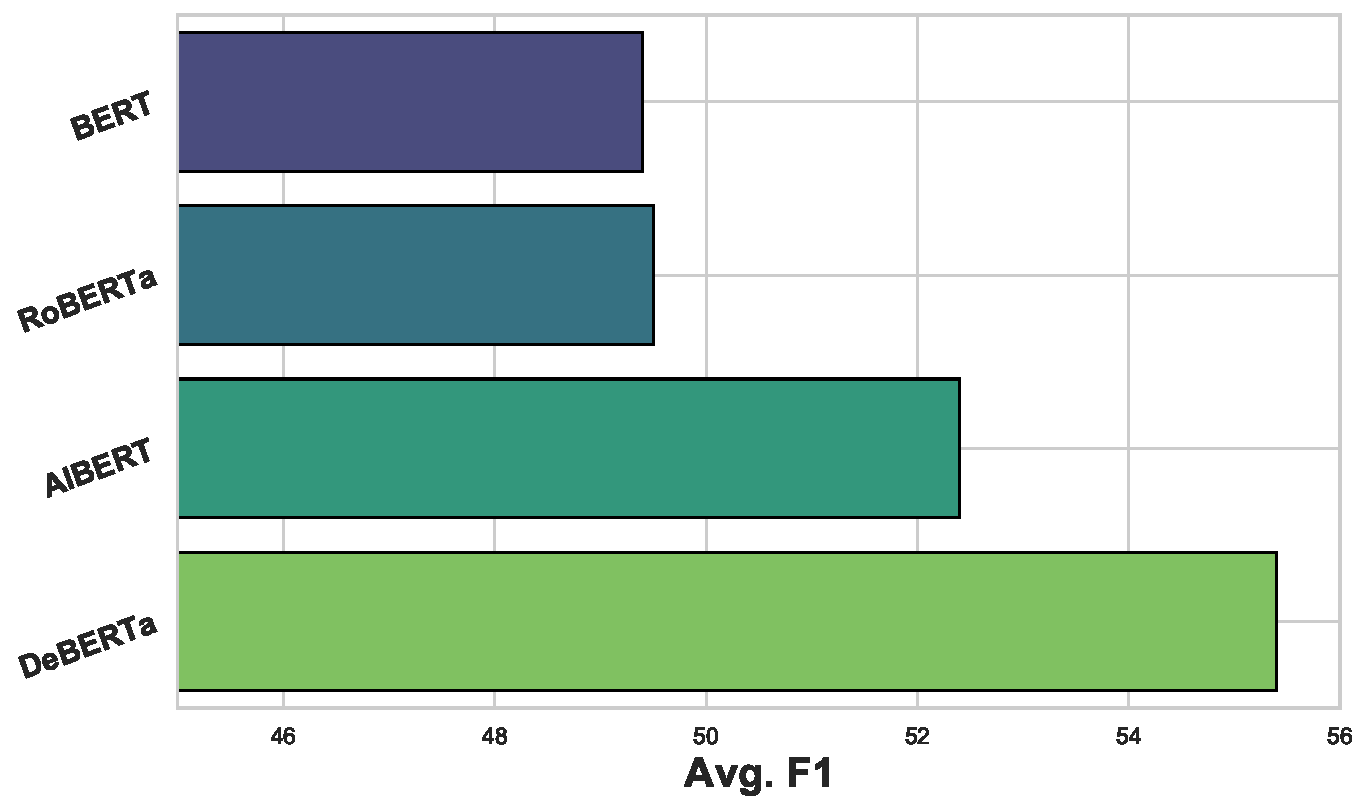
\includegraphics[width=\linewidth]{img/gliner_backbone.pdf}
        \caption{Comparaison des performances des modèles disponibles. Extrait de \cite{zaratiana_gliner_2024}.}
        \label{fig:gliner_backbone}
    \end{minipage}
\end{figure}

La Figure~\ref{fig:gliner_prompt} illustre la structure de la consigne transmise au modèle. Ce format permet de spécifier directement les noms des catégories recherchées sous forme de simples mots-clés, sans modifier le code du programme. Le schéma montre le rôle du message qui fixe la tâche globale, puis la liste des entités cibles. Le texte transcrit est inséré dans le champ d'entrée de la figure précédente pour être analysé.


La Figure~\ref{fig:gliner_backbone} provient des travaux de \citet{zaratiana_gliner_2024}. Les auteurs y évaluent l'impact du modèle de langage sous-jacent sur des jeux de données de référence en extraction d'entités sans réentraînement. La précision y est mesurée par le score F1, une métrique exprimée sur 100 qui combine à la fois la justesse des éléments extraits (la précision) et l'absence d'omissions. Ce graphique permet d'identifier l'architecture la plus efficace pour l'extraction d'informations. On observe que le réseau DeBERTa obtient le meilleur score F1 (55,5), surpassant des architectures comme AlBERT (52,4), RoBERTa (49,5) et BERT (49,4). 

Cependant, cette extraction repose sur la lisibilité du texte. En cas de document très abîmé ou d'écriture illisible, d'autres solutions doivent être envisagées.

\subsection{Les modèles Vision-Langage (VLM)} \label{sec:vlm_execution}


Lorsque certains documents sont très abîmés ou contiennent des mentions mal écrites, les moteurs de lecture par OCR et les modèles d'extraction par mots-clés peuvent atteindre leurs limites. Pour résoudre ces cas, une nouvelle classe d'outils issus de l'intelligence artificielle s'est développée : les modèles Vision-Langage (VLM pour \textit{Vision-Language Models}).

\begin{figure}[H]
    \centering
    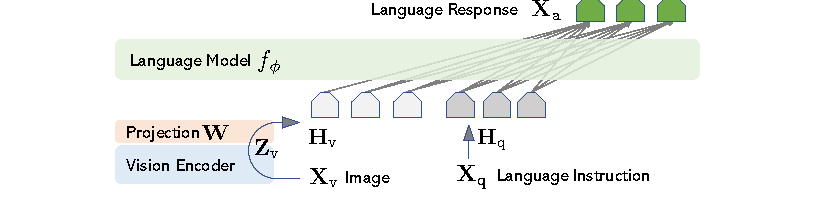
\includegraphics[width=0.85\textwidth]{img/llava_arch.pdf}
    \caption{Architecture interne du modèle Vision-Langage LLaVA. Extrait de \cite{liu_llava_2024}. Une version grand format est disponible en \hyperref[ann:llava_architecture]{Annexe E}.}
    \label{fig:vlm_architecture}
\end{figure}

La Figure~\ref{fig:vlm_architecture} présente l'architecture globale du modèle LLaVA issu des travaux de \citet{liu_llava_2024}. Le fonctionnement du réseau repose sur le couplage d'un encodeur visuel et d'un grand modèle de langage. En bas à gauche du schéma, la photo d'un extrait de document est transmise à l'encodeur visuel (Vision Encoder, fond bleu). Ce composant extrait les caractéristiques visuelles de l'image. Une couche de projection intermédiaire (Projection, fond orange) transforme ensuite ces données visuelles en une suite de représentations numériques compatibles avec le langage. En parallèle, à droite du schéma, la question posée (Language Instruction) est découpée en mots et transformée en texte. Les données visuelles et textuelles sont transmises simultanément au modèle de langage central (Language Model, fond vert), qui génère la réponse finale sous forme de texte.

Ces modèles existent sous deux formes d'exécution distinctes. D'une part, ceux accessibles en ligne (comme GPT-4 Vision ou Claude) proposent de bonnes capacités mais nécessitent le transfert des images vers des serveurs distants. D'autre part, des modèles ouverts et plus légers (comme LLaVA \citep{liu_llava_2024} ou Phi-3 Vision \citep{abdin_phi3_2024}) peuvent être exécutés directement en local sur la machine de l'utilisateur.

D'autres architectures VLM reconnues se distinguent par leur traitement des documents :
\begin{itemize}
  \item \textbf{Donut} \citep{kim_donut_2022} : modèle conçu spécifiquement pour la lecture de documents sans moteur OCR préalable. Ce dernier décode directement l'image pour produire une structure de texte (JSON). Il est plus rapide qu'un VLM classique, mais reste limité aux structures de formulaires connues.
  \item \textbf{Qwen-VL} \citep{bai_qwenvl_2023} : modèle  capable de traiter les images en résolution sans redimensionnement. Cela lui permet de lire de très petits caractères ou des textes denses sur de grands plans sans perte de définition.
  \item \textbf{Phi-3 Vision} \citep{abdin_phi3_2024} : modèle compact optimisé pour l'exécution locale sur un ordinateur standard en découpant les images HD en sous-blocs. Toutefois, comme son entraînement repose quasi exclusivement sur des jeux de données anglophones, ses performances chutent sur du texte en français, surtout pour un vocabulaire technique.
\end{itemize}

Bien que performants pour analyser des visuels de documents, les modèles Vision-Langage présentent deux contraintes. Le temps de calcul par image est plus long que celui d'un modèle d'extraction spécialisé comme YOLO ou GLiNER. De plus, sur des documents dégradés, ces modèles peuvent générer des réponses plausibles mais erronées, un phénomène appelé hallucination.

Dans ce projet, le choix s'est porté sur le modèle ouvert MiniCPM-V exécuté localement sous Ollama. Cette architecture combine un encodeur visuel SigLIP avec un modèle de langage compact. L'image de la zone d'intérêt est découpée en trames visuelles transformées en jetons textuels, permettant au réseau de répondre à des consignes ciblées en français. Pour réduire le temps de réponse et l'occupation mémoire, les poids du modèle ont été quantifiés en 4 bits, rendant l'inférence possible sur les processeurs graphiques standards du cabinet sans compromettre la compréhension des écritures manuscrites.



% A RELIRE
\subsection{La détection et l'extraction de tableaux dans les documents}
\label{subsec:table_detection}

Beaucoup de documents administratifs organisent leur contenu en colonnes et en lignes. Repérer la structure d'un tableau dans une image et en extraire le contenu est un problème distinct de la simple lecture de texte. Ce problème a été étudié depuis les travaux de \citet{duda_hough_1972} sur la détection de lignes géométriques.

Les premières approches reposent sur la transformée de Hough~\citep{duda_hough_1972}, qui repère les lignes horizontales et verticales dans l'image pour en déduire la grille du tableau. Cette technique fonctionne sur les tableaux imprimés dont les traits sont continus. En revanche, sur les documents anciens, les lignes de colonnes sont souvent discontinues ou absentes, remplacées par un simple alignement visuel des mots sans séparateur. \citet{canny_edge_1986} ont étendu cette approche par une détection préalable des contours, mais la limite sur les documents dégradés reste la même.

Des modèles entraînés à reconnaître la structure des tableaux ont ensuite été proposés. Le modèle \textit{Table Transformer} (TATR) de \citet{smock_table_2022} repose sur une architecture DETR (\textit{Detection Transformer}). Il analyse directement l'image et prédit la position de chaque ligne et colonne sous forme de boîtes englobantes, sans règles géométriques fixées à l'avance. Entraîné sur les jeux de données PubTables-1M et FinTabNet, il atteint un score F1 supérieur à 0,97 sur des tableaux imprimés normalisés. \citet{chi_complicated_2019} s'intéressent aux tableaux avec des cellules fusionnées et montrent que les architectures par décodage de graphe surpassent les approches par détection d'objets sur ces configurations.

\begin{figure}[H]
    \centering
    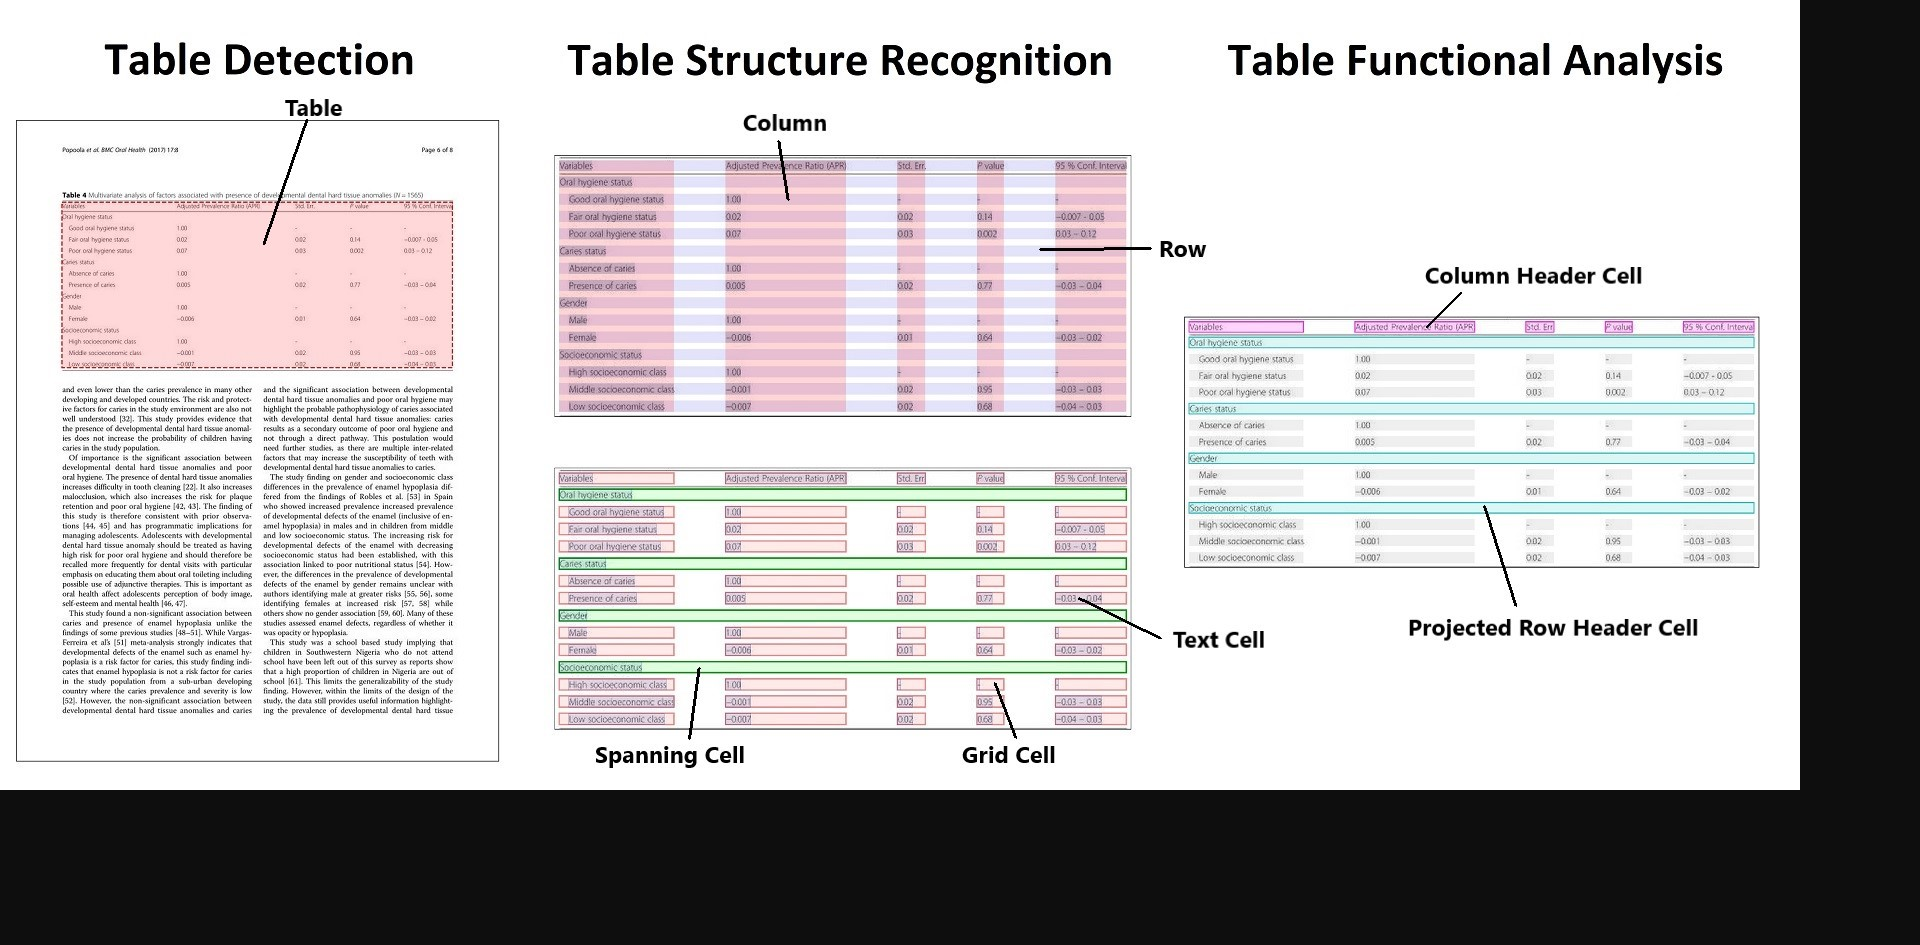
\includegraphics[width=\textwidth]{img/table_transformer_overview.png}
    \caption{Les trois tâches du Table Transformer de \citet{smock_table_2022} : détection de la table dans la page (gauche), reconnaissance de sa structure en lignes et colonnes (centre), et analyse fonctionnelle des types de cellules (droite). Source : \citet{microsoft_tatr_github}. Une version grand format est disponible en \hyperref[ann:table_transformer]{Annexe F}.}
    \label{fig:table_detection_overview}
\end{figure}

Sur des documents anciens numérisés à basse résolution, ces modèles se heurtent aux mêmes problèmes que les méthodes classiques. Les cellules ne sont parfois séparées que par un espace, et les plis du papier peuvent être lus à tort comme des séparateurs. \citet{zhong_image-based_2019} montrent que la position spatiale des blocs de texte, combinée à une analyse des proximités horizontales et verticales, est une alternative robuste quand les séparateurs visuels sont absents.

Dans les registres d'archives historiques où la séparation des colonnes repose sur un alignement visuel, l'analyse de la densité horizontale des projections de texte permet de détecter les espacements (zones blanches verticales). L'algorithme calcule l'histogramme des projections verticales des boîtes de texte sur la largeur de la page et identifie les creux de densité correspondant aux séparations naturelles entre les colonnes de données.

Pour compenser les décalages de ligne sur les registres, les coordonnées verticales des centroïdes des blocs de texte sont regroupées par un algorithme de clustering unidimensionnel (DBSCAN). Ce regroupement permet de rattacher chaque mot à sa ligne d'origine même si le rédacteur a écrit de manière oblique ou non rectiligne.

Cette analyse de la mise en page des tableaux est importante pour exploiter les répertoires d'anciens géomètres, comme présenté au chapitre~\ref{sec:architecture}. Elle permet l'alignement des données avant d'alimenter les modules suivants du projet.


Dans ce projet, les documents traités se répartissent en deux cas. Les formulaires DMPC imprimés ont des cases délimitées par des traits continus : la détection par boîtes englobantes via YOLOv8 suffit (chapitre~\ref{sec:architecture}). Les registres manuscrits, eux, organisent les données en colonnes sans trait visible. Dans ce second cas, ni la transformée de Hough ni le Table Transformer ne s'appliquent directement. La solution retenue combine la détection des blocs de texte par EasyOCR et leur regroupement par proximité verticale, comme détaillé pour la numérisation des registres au chapitre~\ref{sec:fiabilisation}.


\subsection{Métriques d'évaluation de la reconnaissance de texte}
\label{subsec:metrics_ocr}

Pour comparer les performances des modèles d'OCR, de HTR et d'extraction d'entités, la littérature scientifique s'appuie sur plusieurs métriques standardisées.

Le taux d'erreur sur les caractères (\textit{Character Error Rate} ou CER) mesure la proportion de caractères mal transcrits par rapport à la vérité terrain. Il repose sur la distance de Levenshtein au niveau des caractères :

\begin{equation}
  \text{CER} = \frac{S + D + I}{N}
\end{equation}

où $S$ est le nombre de substitutions, $D$ le nombre de suppressions, $I$ le nombre d'insertions et $N$ le nombre total de caractères dans le texte de référence. Un CER de 0\,\% indique une transcription parfaite, tandis qu'un CER inférieur à 5\,\% est considéré comme bon pour du texte manuscrit.

Le taux d'erreur sur les mots (\textit{Word Error Rate} ou WER) s'appuie sur le même principe, mais calculé au niveau des mots complets :

\begin{equation}
  \text{WER} = \frac{S_w + D_w + I_w}{N_w}
\end{equation}

où $S_w$, $D_w$ et $I_w$ représentent respectivement les substitutions, suppressions et insertions de mots entiers, et $N_w$ le nombre total de mots. Le WER est plus sévère que le CER, car une seule lettre de différence rend le mot entier faux.
% >>>>>>>>>>>>>>>>>>>

\textbf{Précision, Rappel et Score F1.} Pour l'extraction d'entités (comme la détection des noms de communes ou des numéros de parcelles par GLiNER), les métriques habituelles sont la précision ($P$), le rappel ($R$) et le score F1 ($F_1$) :

\begin{equation}
  P = \frac{TP}{TP + FP}, \quad R = \frac{TP}{TP + FN}, \quad F_1 = 2 \times \frac{P \times R}{P + R}
\end{equation}

où $TP$ désigne les vrais positifs (entités correctement extraites), $FP$ les faux positifs (entités attribuées à tort) et $FN$ les faux négatifs (entités manquées). Le score F1 combine précision et rappel en une valeur unique comprise entre 0 et 1 (ou 0\,\% et 100\,\%).
% >>>>>>>>>>>>>>>>>>>


\subsection{Synthèse des approches de l'état de l'art}




Chaque technologie étudiée dans ce chapitre répond à une tâche précise de l'analyse de document, qu'il s'agisse d'isoler des zones, de lire du texte ou d'en comprendre le sens. Le Tableau~\ref{tab:comparaison_modeles} regroupe ces différentes méthodes afin de comparer leur fonctionnement, leurs avantages et leurs limites, avec pour objectif de selectionner le plus propice au cas d'étude.

\begin{table}[H]
  \centering
  \small
  \renewcommand{\arraystretch}{1.35}
  \resizebox{\textwidth}{!}{%
  \begin{tabular}{@{} l p{3.4cm} c p{4.2cm} p{4.2cm} @{}}
    \toprule
    \textbf{Modèle} & \textbf{Méthode utilisée} & \textbf{Ressources} & \textbf{Points forts} & \textbf{Limites principales} \\
    \midrule
    Tesseract v5 & Analyse par caractères & CPU & Rapide et économe en mémoire. & Précision très faible sur le manuscrit. \\
    
    PyLaia / TrOCR & Réseau convolutif et Transformer & ~4 Go GPU & Forte précision sur le manuscrit. & Nécessite d'isoler les lignes au préalable. \\
    
    YOLOv8 & Détection d'objets spatiale & < 2 Go GPU & Détection visuelle très rapide et robuste. & Isole les zones sans lire le texte. \\
    
    LayoutLMv3 & Modèle multimodal vision-texte & ~8 Go GPU & Analyse conjointe de la forme et des mots. & Sensible aux erreurs de lecture initiale. \\
    
    GLiNER & Comparaison de représentations & ~2 Go GPU & Identification d'entités sans réentraînement. & Dépend de la propreté du texte transmis. \\
    
    Donut & Décodage visuel direct  & ~4 Go GPU & Extraction  sans OCR externe. & Limité aux types de fichiers connus. \\
    
    Qwen-VL & VLM à résolution dynamique & ~8 Go GPU & Lecture précise des détails et petits textes. & Temps de calcul élevé sur grand format. \\
    
    LLaVA / Ollama & Modèle Vision-Langage local & > 8 Go GPU & Raisonnement visuel direct en local. & Calcul lent et risque d'hallucination. \\
    \bottomrule
  \end{tabular}%
  }
  \caption{Synthèse comparative des technologies d'analyse de documents.}
  \label{tab:comparaison_modeles}
\end{table}

Pour comparer ces outils, il faut prendre en compte la machine de test. L'ensemble des essais s'appuie sur une configuration standard équipée d'un processeur Intel Core i7, de 32 Go de RAM et d'une carte graphique NVIDIA de 8 Go (VRAM), ce matériel constitue le cas d'étude, la puissance variant que très légèrement entres les postes du cabinet. 

Cette configuration matérielle influence directement le choix des modèles du Tableau~\ref{tab:comparaison_modeles}. Les outils légers comme YOLOv8 et GLiNER occupent moins de 2 Go de mémoire graphique et répondent presque instantanément. PyLaia utilise environ 4 Go pour lire une ligne en moins d'une seconde. À l'inverse, les modèles plus lourds comme LayoutLMv3 et LLaVA demandent beaucoup plus de ressources. Avec Ollama, LLaVA prend environ 4,8 secondes par extrait. De plus, son risque principal reste l'hallucination : sur un texte très abîmé, le modèle a parfois tendance à inventer une réponse crédible au lieu de signaler qu'il n'arrive pas à lire.

Pour compléter ces observations, la Figure~\ref{fig:benchmark_comparatif} compare la précision de chaque méthode (en bleu) et son temps de traitement moyen par zone (en orange). Ces valeurs sont issues des tests présentés dans les articles scientifiques sur des formulaires administratifs, des registres manuscrits et des documents de référence.

\begin{figure}[H]
    \centering
    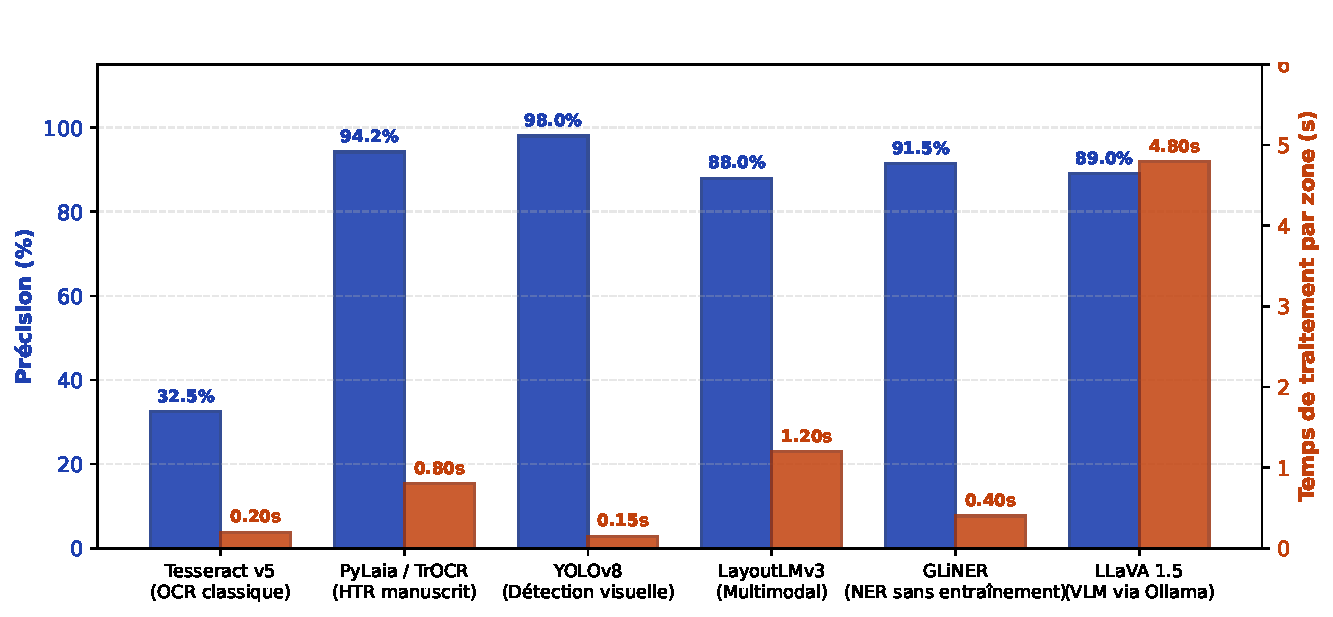
\includegraphics[width=0.92\textwidth]{img/benchmark_comparatif_modeles.pdf}
    \caption{Graphique comparatif de la précision et du temps de traitement moyen par zone selon les architectures étudiées (\cite{smith_tesseract_2007}, \cite{li_trocr_2021}, \cite{jiang_review_2022}, \cite{bajrami_comprehensive_2023}, \cite{zaratiana_gliner_2024}, \cite{liu_llava_2024}).}
    \label{fig:benchmark_comparatif}
\end{figure}

YOLOv8 se montre très rapide (0,15 seconde par zone) et efficace pour repérer les emplacements (98,0\%). Il permet d'isoler rapidement les tampons, les signatures ou les tableaux sans lire le texte. À l'opposé, un modèle comme LLaVA demande environ 4,80 secondes par zone en local. Comme expliqué dans la Section~\ref{sec:vlm_execution}, l'utilisation de services en ligne pose la question de la confidentialité des données d'archives. Même si LLaVA obtient 89,0\% de réussite grâce au raisonnement visuel direct, ce temps de calcul élevé constitue sa limite principale sur des volumes importants de documents.

L'analyse des articles de la littérature confirme ces résultats. Les moteurs de lecture classiques comme Tesseract \citep{smith_tesseract_2007} fonctionnent bien sur des imprimés propres, mais leur taux d'erreur dépasse 30\% dès que le texte est manuscrit. À l'inverse, les modèles de reconnaissance manuscrite (HTR) comme TrOCR \citep{li_trocr_2021} et PyLaia \citep{tarride_improving_2024} lisent très bien l'écriture manuelle (moins de 6\% d'erreur, d'après la synthèse de \citet{alkendi_advancements_2024}), mais ils exigent que le texte leur soit transmis ligne par ligne.

Pour découper ces lignes sans problématiques de mise en page, la détection avec YOLOv8 \citep{redmon_yolo_2016, jiang_review_2022} permet d'isoler proprement chaque zone de texte avant la lecture.


Du côté de la compréhension du texte, les modèles comme LayoutLM \citep{xu_layoutlm_2020} essaient d'analyser à la fois la forme et les mots. Cependant, les travaux comparatifs de \citet{bajrami_comprehensive_2023} montrent que LayoutLM reste très sensible aux fautes de lecture de l'OCR : dès que le texte extrait contient des erreurs, la compréhension globale baisse nettement (autour de 88,0\% au mieux). C'est ce qui a poussé les chercheurs à développer des modules de correction comme LayoutLM-Critic \citep{xu_layoutlm-critic_2022}.

De leur côté, des outils comme GLiNER permettent d'extraire des entités (communes, dates, parcelles) sans réentraînement, avec un score F1 de 91,5\%, à condition que le texte fourni soit propre.

Cette analyse montre qu'aucune technologie existante ne peut traiter seule l'ensemble des archives du projet. L'OCR classique échoue sur l'écriture manuscrite, les modèles HTR exigent un découpage préalable des lignes, LayoutLM reste bloqué par les erreurs de lecture, et les VLM demandent trop de temps de calcul. C'est pourquoi il convient d'associer plusieurs de ces approches au sein du projet, en utilisant chaque outil uniquement là où il est le plus efficace (chapitre~\ref{sec:architecture}).


\subsection{Choix des méthodes retenues}

Afin de répondre aux contraintes du projet et de trouver une solution pour minimiser les limites de chaque modèle, une méthode combinant quatre outils a été retenue :

\begin{itemize}
  \item Ultralytics YOLOv8 pour la segmentation spatiale : ce modèle découpe visuellement les zones d'intérêt sur les formulaires imprimés sans dépendre du texte.
  \item EasyOCR et PyLaia pour l'extraction textuelle : EasyOCR lit les parties imprimées tandis que PyLaia traite l'écriture manuscrite des registres.
  \item GLiNER pour le repérage des entités : il identifie les champs clés (commune, date, section, parcelles) dans le texte extrait sans réentraînement préalable.
  \item Ollama avec MiniCPM-V en secours local : ce modèle VLM s'exécute uniquement sur les zones incertaines pour lever les ambiguïtés de lecture.
\end{itemize}

Cette architecture hybride garantit le respect du secret professionnel en fonctionnant intégralement en local (chapitre~\ref{sec:analyse_metier}). Elle prépare les données pour la phase de fiabilisation et de validation par l'opérateur (chapitre~\ref{sec:fiabilisation}), avant l'exportation vers le portail Géofoncier (chapitre~\ref{sec:integration}).


Pour le repérage des zones, le modèle YOLOv8 a été choisi. Son rôle est d'isoler les cases des communes, les dates, les tableaux de parcelles ainsi que les tampons permettant d'identifier le géomètre-expert ayant réalisé la mission. Ce choix s'explique par sa rapidité (0,15 seconde par zone), sa faible consommation de mémoire graphique (moins de 2 Go) et son insensibilité au texte. Il permet de découper proprement les images sans dépendre d'un gabarit fixe, et de préparer ainsi les extraits d'images nécessaires au fonctionnement du modèle PyLaia.


Pour la transcription du texte manuscrit, le modèle HTR PyLaia a été sélectionné. Alors que l'OCR classique comme Tesseract échoue sur l'écriture manuelle, PyLaia lit les registres manuscrits avec précision dès que les lignes lui sont transmises sous forme de découpes isolées par YOLO.

Pour l'extraction des données clés (noms de communes, dates, numéros de parcelles), l'outil GLiNER a été retenu. Contrairement aux modèles comme LayoutLM qui deviennent inefficaces lorsque le texte contient des fautes, GLiNER identifie les entités sans entraînement spécifique et réduit le risque de faux positif, comme présenté dans ce chapitre.

Le détail de l'implémentation de chacun de ces outils et leur enchaînement dans la chaîne de traitement sont détaillés au chapitre~\ref{sec:architecture}.




